\documentclass[12pt]{ucthesis}

\usepackage{etex}
\usepackage[morefloats=125]{morefloats}
\usepackage[hyphens]{url}
\usepackage[breaklinks=true]{hyperref}
\usepackage{subfig}
\usepackage{graphicx}
\usepackage{tabularx}
\usepackage{amssymb}
\usepackage{amsmath}
\usepackage[letterpaper]{geometry}
\usepackage[overload]{textcase}
\usepackage{color}
\usepackage[nonumberlist,toc]{glossaries}
\usepackage{wrapfig}
\usepackage{longtable}
\usepackage{morefloats}
\usepackage{float}
\usepackage{listings}
\usepackage{makecell}
\usepackage[titletoc]{appendix}
\usepackage{cleveref}
\usepackage[]{algorithm2e}
\usepackage{fancyvrb}

\makeindex
\makeglossaries

\bibliographystyle{abbrv}

\setlength{\parindent}{0.25in} \setlength{\parskip}{6pt}
\geometry{verbose,nohead,tmargin=1in,bmargin=1in,lmargin=1.5in,rmargin=1in}
\setcounter{tocdepth}{2}

% Different font in captions (single-spaced, bold) ------------
\newcommand{\captionfonts}{\small\bf\ssp}

\newcommand{\mycaption}[2]{\caption[#1 --- #2]{#1 --- #2}}

\makeatletter  % Allow the use of @ in command names
\long\def\@makecaption#1#2{%
  \vskip\abovecaptionskip
  \sbox\@tempboxa{{\captionfonts #1: #2}}%
  \ifdim \wd\@tempboxa >\hsize
    {\captionfonts #1: #2\par}
  \else
    \hbox to\hsize{\hfil\box\@tempboxa\hfil}%
  \fi
  \vskip\belowcaptionskip}
\makeatother   % Cancel the effect of \makeatletter
% ---------------------------------------

% Define Appendix refs
\crefname{app}{appendix}{appendices}
\Crefname{app}{Appendix}{Appendices}

\begin{document}

% Declarations for Front Matter
\title{Geospatial Data Modeling to Support Energy Pipeline Integrity Management}
\author{Austin Wylie}
\degreemonth{June} \degreeyear{2015} \degree{Master of Science}
\defensemonth{June} \defenseyear{2015}
\numberofmembers{3}
   \chair{Professor Alexander Dekhtyar, Ph.D. \linebreak Department of Computer Science}
   \othermemberA{Professor Christopher Lupo, Ph.D. \linebreak Department of Computer Science}
   \othermemberB{Professor Gene Fisher, Ph.D. \linebreak Department of Computer Science}
\field{Computer Science} \campus{San Luis Obispo}
\copyrightyears{seven}

\maketitle

\begin{frontmatter}

% Custom made for Cal Poly (by Mark Barry, modified by Andrew Tsui).
\copyrightpage

% Custom made for Cal Poly (by Andrew Tsui).
\committeemembershippage

\begin{abstract}
Several hundred thousand miles of energy pipelines span the whole of North America---responsible for carrying the natural gas and liquid petroleum that power the continent's homes and economies~\cite{PHMSA}. These pipelines, so crucial to everyday goings-on, are closely monitored by various operating companies to ensure they perform safely and smoothly~\cite{PHMSA2013}. 

Happenings like earthquakes, erosion, and extreme weather, however---and human factors like vehicle traffic and construction---all pose threats to pipeline integrity. As such, there's a tremendous need to measure and indicate useful, actionable data for each region of interest, and operators often use computer-based decision support systems (DSS) to analyze and allocate resources for active and potential hazards~\cite{PHMSA2013,MichaelBakerJr.2008,Chastain,Dunning2013}.

We designed and implemented a geospatial data service, \textit{REST API for Pipeline Integrity Data} (RAPID) to improve the amount and quality of data available to DSS. More specifically, RAPID---built with a spatial database and the Django web framework---allows third-party software to manage and query an arbitrary number of geographic data sources through one centralized REST API.

Here, we focus on the process and peculiarities of creating RAPID's model and query interface for pipeline integrity management; this contribution describes the design, implementation, and validation that model, which builds on existing geographic standards.
\end{abstract}

\begin{acknowledgements}
\noindent
My thesis would not be what it is today (read: finished) without invaluable support and instruction from many people. This group has my deepest thanks:
\begin{itemize}
    \item Dr. Alex Dekhtyar for advice, encouragement, and knowledge to work with biologists.
    \item Dr. Chris Lupo for teaching me to throw hardware at the problem. And the Picture of the Day.
    \item Alexa Francis---a solid classmate and neighbor---for learning about Web Feature Services with me.
    \item My parents, Suzi and Patrick, for academic cheerleading and a bunch of love.
\end{itemize}
\end{acknowledgements}

\tableofcontents

\listoftables

\listoffigures

\end{frontmatter}

\pagestyle{plain}

\renewcommand{\baselinestretch}{1.66}

\chapter{Changelog and Notes}
\label{intro}

\paragraph{Past tense versus present tense?}


SRID 4326\footnote{As further explanation of our ability to interchange ``spatial'' and ``geospatial,'' we could use \textit{any} coordinate system, but }
Design decision

Citations are sparse
\chapter{Introduction}
\label{intro}

\section{Problem definition}
\label{Problem}
Several hundred thousand miles of energy pipelines span the whole of North America---responsible for carrying the natural gas and liquid petroleum that power the continent's homes and economies~\cite{PHMSA}. These pipelines, so crucial to everyday goings-on, are closely monitored by various operating companies to ensure they perform safely and smoothly~\cite{PHMSA2013}.

Happenings like earthquakes, erosion, and extreme weather---and human factors like vehicle traffic and construction---all pose threats to pipeline integrity~\cite{MichaelBakerJr.2008,Chastain,Dunning2013}. Compromised lines put business activities at risk; individual safety, personal property, and the surrounding environment feel the impacts as well~\cite{Dunning2013}. However, with appropriate knowledge and management processes, these issues can be avoided~\cite{Dunning2013,Chastain}.

As such, there is a tremendous need to measure and indicate useful, actionable data for each region of interest. It is difficult, though, to keep a close-enough eye on massive pipeline networks with manual, in-person inspections~\cite{Dunning2013,Chastain}. Even recurring aerial surveillance demands too much information from too few (and distant) sources~\cite{Dunning2013}.

As an alternative to visiting pipeline sites, operators often use computer-based decision support systems (DSS) to learn about and allocate resources for active and potential hazards~\cite{PHMSA2013,Dunning2013}. 

In general, these DSS allow operators to coalesce and study geographic, demographic, and remote sensor data relevant to pipeline integrity management~\cite{RedlandsSDSS,Dunning2013}. A great deal of worthwhile DSS data is already recorded, stored, and made available for analysis, but it is scattered across physical and digital media and locations. As such, pipeline operators are left to pick and choose smaller subsets of attainable and manageable inputs for analysis, which can end up painting an incomplete picture~\cite{Dunning2013}.

\section{Contributions}
We have created specific system requirements alongside web developers and industry partners to address their primary data aggregation and analysis needs. The remainder of this document describes the implemented, deployed, and validated software for improving the amount and quality of data available to pipeline operator DSS, which we dubbed \textit{REST API for Pipeline Integrity Data} (RAPID). More specifically, RAPID allows third-party applications to manage and query an arbitrary number of disparate geographic data sources through one REST API. Rather than leaving DSS and their users to identify, model, convert between, and store dozens of data formats and repositories, our system manages and hides that trivia---instead exposing simple REST calls for more consistency and centralization.

A lot of geospatial data is conceptually alike because it pairs a physical location or demarcation with information about that place. The crux of the problem from Section~\ref{Problem}, though, is that there are numerous and varied formats and access methods for those geospatial datasets. However, with appropriate modeling and processing, they can each be stored, modified, and queried in approximately the same way.

As we built it, RAPID uses the Python-based Django web framework with a PostgreSQL database. To store and query first-class geospatial data, PostgreSQL's PostGIS extension has been added and enabled, and our schema stores geometries and metadata located on Earth's surface.

Our most significant contribution to this project was the design and implementation of RAPID's data model (along with supplementary tools). In this document, we describe the process and peculiarities of building the RAPID model and query interface for real-world pipeline integrity management.

While the database itself is not accessible to external users, developers and applications can interact with the aggregated content through a well-defined REST API.\footnote{REST, or \textit{Representational State Transfer} is an architectural style for web service APIs, often using HTTP~\cite{Francis}.} The API provides means of looking up geospatial data for particular regions (in space and time), as well as necessary metadata and documentation for its use and interpretation.

As a crude example, this allows API users to make a request like ``retrieve all rain data for California in JSON'' as well as a request like ``retrieve all \textit{seismic} data for California in JSON \textit{from last week}.'' The rain data may have originated as JSON files from portable weather stations; the seismic data could have come from a Shapefile on a government server.\footnote{We discuss particulars for RAPID's supported formats in the following chapters.} The point is that customers can view and download different forms of data from wildly different sources in a mostly-standard and interchangeable fashion.

My research partner, Alexa Francis, focuses on the REST API in her master's thesis, covering its implementation and usage, with considerations for third-party developers and our internal system architecture~\cite{Francis}.

\label{polyview_intro}
Finally, serving to validate our system, an external web application has been built to use RAPID---both retrieving and visualizing geospatial data. This additional software, RAPID UI, aggregates and indexes several datasets relevant to our pipeline operating partners and displays \textit{a}) how they are organized within our system and \textit{b}) where and what the geospatial features are.

RAPID UI looks up important locations and associated properties using the RAPID API, letting the UI perform quick and easy location-based queries with only HTTP requests---normally requiring custom-built logic for spatial processing. We have also used RAPID UI's activities to guide performance measurements and optimization. While our own test data does not strain RAPID as much as a pipeline-covered continent would, we also show system efficiency and stability during real, on-demand work.

\paragraph{Document outline.}
Following this chapter, Chapter~\ref{background} discusses the most essential and helpful context for creating RAPID, including related software, standards, and theory. Chapter~\ref{requirements} overviews our guiding set of system requirements---coming from partners and commonplace industry recommendations. Chapter~\ref{design} shows how we built RAPID, designing the data model and algorithms in Python. Chapter~\ref{validation} describes our procedure for validating RAPID, showing a correct and efficient implemented solution. Chapter~\ref{conclusions} concludes this document, summarizing our work and other contributions that may follow.


% \subsection{Data Management Dashboard}
% Lastly, a web dashboard for data management was created for customers, which lets them add, update, and remove tracked geospatial features. When someone points the dashboard at an input dataset, it is cleaned, parsed, and added to the integrated database. The user interface and application functionality are robust and friendly enough to handle the most common input formats, and they allow for intuitive viewing and modification of previously-added data.
\chapter{Background}
\label{background}

\section{Introduction}
\label{background_intro}
RAPID's connected DSSs make use of spatial data;\footnote{\textit{Spatial} versus \textit{geospatial} terminology: Some groups make a subtle distinction between spatial data and geospatial data. In those cases, spatial data describes data ``distributed in three-dimensional space,'' with ``measurable'' dimensions~\cite{Bhatta2011}. Given \textit{geography}'s definition, geospatial data is ``spatial data which is related to the Earth''~\cite{Bhatta2011}. In this thesis, spatial data is always located on Earth, so \textit{spatial} and \textit{geospatial} will be used interchangeably. As one supporting source, the United States Geological Survey considers ``the terms spatial and geospatial [to be] equivalent.''
\cite{Bhatta2011}} their eventual goal is to lay out and recommend pipeline routes through areas with as few hazards as possible~\cite{Dunning2013}. As such, this end-to-end system can be considered a spatial DSS (SDSS). SDSSs are uniquely tasked with providing ``easy access to spatial data and decision models through the integration of spatial databases, analytical models, and visualization tools''~\cite{RedlandsSDSS}.

RAPID manages the spatial database component and also has to account for geographic information systems' (GIS) mathematical foundations. This chapter describes basic GIS concepts and requisite information for geospatial database management systems, structured and unstructured geospatial data, and related standards. These have all played into RAPID's motivations and implementation.

\subsection{Open Geospatial Consortium}
The Open Geospatial Consortium (OGC) is an international consortium---originating in 1994---with several hundred industry, government, and academic participants. Its goal is to establish standard formats and interfaces for geospatial data and applications. They've created over thirty-five standards, usually in the form of markup, modeling, or query languages as well as API specifications~\cite{ogc}.

Many organizations insist on using OGC-compliant products and services to promote robustness and interoperability. RAPID implements components of several OGC Standards. While not a top-to-bottom OGC-standardized system, RAPID is partway there and still useful because it builds on the same foundational concepts.

\section{GISs}
A GIS is a computer system (including hardware and software) for working with geographic data---that is, data associated with a location in space~\cite{Esriintro}. Quite simply, GISs provide a means of managing and analyzing this data. More importantly, GISs allow people to understand deep, complex information about geographic locations, their relative positions, and the objects and conditions that are located there~\cite{Esriintro}.

Because many everyday and large-scale tasks and concerns are related to specific locations, so too are the computer applications that people use: flight scheduling and routing, car navigation, weather prediction, demographic analysis, social networking, economics, and politics~\cite{Esriintro}. RAPID and its related applications, with their geospatial data, enable similar uses.

\subsection{Functionality}
GIS functionality can usually be placed in one of five categories~\cite{Esriintro}:

\begin{description}
  \item[Mapping objects' locations] Descriptors can be assigned to points in space: for example, addresses. In a technical sense, this can usually be seen as associating string-like data---ideas or concepts (like place names)---with floating-point latitude and longitude. These are commonly called \textit{features} (central to any geospatial system).
  \item[Mapping quantities] Quantities can be mapped to certain points to relate locations to numeric data about them. This could be integers and floating point values, again, assigned to latitude and longitude. These can also be considered features.
  \item[Mapping densities] Not only can values be assigned to specific points on a map, densities can be generated and displayed, which show the distribution of objects or values over an area.
  \item[Determining objects' relative positions] GISs can determine if objects or locations are located inside or outside of other locations. Additionally, they measure distances between objects and locations and determine how near or far objects are.\footnote{This is the key to geospatial database management system design---looking up data based on spatial calculations quickly.}
  \item[Analyzing trends] Lastly, many GISs look at trends in data. There's a lot of demand and opportunity for analysis of how locations and features change over time.
\end{description}

In summary, GISs capture, manage, analyze, and display geographically-referenced information. Viewing and understanding relevant relationships, patterns, and trends can be done in the form of maps, globes, reports, and charts~\cite{Esriintro}. RAPID, at a low level, acts as a foundation for that functionality.

\section{Data characteristics}
The section outlines more technical design considerations for geospatial data, which isn't always easily represented or stored in common data formats. Although humans often represent points in space with numbers (and, occasionally, symbols) it's best to treat them as their own primitive data type in software~\cite{gentle_intro}.

Because of this, geospatial data structures and file formats must be able to specify points in two or three dimensions (usually latitude and longitude, and maybe elevation).\footnote{Conceptually, time can be viewed as an additional dimension---one of a feature's properties---so the data is geospatial-\textit{temporal}.} GISs and spatial database management systems often need to account for any arbitrary coordinate system~\cite{gentle_intro}.

Considering the above, two common file and data types have come about in GISs: vector and raster. They are briefly described below.

\subsubsection{Vector}
\label{sec:vector}
Vector files contain mathematical and geometric representations of spatial data---defining points and shapes in space. They are split into two components: (1) series of coordinate pairs and (2) attributes~\cite{gentle_intro}.

\paragraph{Coordinate pair series}
Coordinate pairs are two values that represent a point in space in a coordinate system. Most commonly, this is the geographic coordinate system, where one value is latitude and other value is latitude. Taken together, any point on Earth's surface can be represented~\cite{gentle_intro}.\footnote{Geographic projections and digital coordinate system specifications are a large area of study. RAPID cannot entirely ignore these considerations and distinctions, but once a few database and parser options are set, we can mostly set those concerns aside. This is discussed in Section~\ref{design_srid}.}

In vector files, sequences (or ``series'') of these points can represent different cartographic concepts. There are points, lines, linestrings, and polygons:

\begin{description}
  \item[Points] Points are single instances of the points described above: they represent a single point in space.
  \item[Lines] Lines are drawn from one point to another (and are represented by that pair of points).
  \item[Linestrings] Linestrings are multiple connected lines (and, thus, chained pairs of points). These can represent concepts like borders between countries or road networks.
  \item[Polygons] Polygons are linestrings where the last point is equal to the first point---creating a closed shape. Political borders in the United States are a good example: the country is broken up into states, and states are broken up into counties, cities, and congressional districts.
\end{description}

The above can be extended to include polygons with holes. Imagine mapping California's land: where there are bodies of water on the map, there are simply holes in the polygon~\cite{gentle_intro}.

\paragraph{Attributes}
Attributes are simply non-spatial data that's associated with the spatial data described above. An address, as mentioned above, is a great example of this: house numbers, streets, city, state, and zip code all associate an identifier with a point in space or other spatial concept (likely both!)~\cite{gentle_intro}.

\subsubsection{Raster}
Raster data is simply made up of grids of values. It's best to imagine a digital image: pixels arranged in a grid are each assigned red, green, and blue color values, and when they're appropriately combined and visualized, a continuous dataset is spread over a grid in two or three dimensions~\cite{gentle_intro}.

Images, in fact, are often raster data found in GISs, like satellite images. Atmospheric or ground sensors can also provide data sets that blanket an area~\cite{gentle_intro}.

Because raster data covers an area, programs and users need to account for the \textit{density} of data---that is, the size of each grid cell, which is referred to as the ``resolution.'' Resolution is either \textit{spatial} or \textit{spectral}:

\begin{description}
  \item[Spatial] Spatial resolution is how large a cell of the grid is and how it corresponds to a real geographic area. For example, a side of one cell could be four feet.
  \item[Spectral] Spectral resolution is the number of color ``bands'' in raster images. In an ordinary image, red, green, and blue are these three bands---the spectral resolution. In some cases, images may also capture infrared or ultraviolet light and store more data in other color bands.
\end{description}

\paragraph{Georeferencing}
Georeferencing makes raster data useful geographically: it associates the raster data with a location. For example, a GIS that displays a satellite image of California on top of an interactive state map can calculate where real geographic features are in the image~\cite{gentle_intro}.

As long as four pieces of information are known, a raster file can be properly georeferenced:

\begin{itemize}
  \item Coordinates of the file's top-left pixel
  \item Width of a pixel
  \item Height of a pixel
  \item Rotation of the grid
\end{itemize}

These four values will accurately positioned in a coordinate system~\cite{gentle_intro}.

\subsection{Abstract Specification}
OGC's Abstract Specification describes and standardizes the essential components of geospatial data, including the central information model and glossary for all OGC Standards~\cite{AbstractSpecFaq}.

Any sizable geospatial software system is naturally governed by certain geographic and geometric properties and functions; the Abstract Specification is the OGC's formalization of those concepts, all of which are encompassed in the data types and formats above and below~\cite{AbstractSpecFaq}.

\section{Data storage}
This section overviews several storage considerations for GIS data.

\subsection{Geospatial database management systems}
Because of the unique data considerations described earlier, databases that manage geospatial data need to pay special attention to the methods of doing so. Geospatial database management systems (GDBMSs) provide ways of storing and querying geospatial data. This includes syntax for adding vector and raster data types.

\paragraph{Example}
\label{background_wkt}
Inserting geometries (vector data) into a GDBMS can look like the following. We are using a SQL statement to add a point, linestring, polygon, and polygon with a hole to a PostGIS database (RAPID's underlying DBMS).

Note that space-separated numbers are a coordinate pair. The commas separate the points, creating an ordered series. This particular syntax is Well-Known Text (WKT), an OGC Standard for defining Abstract Specification geometries~\cite{ogc}. The five geometric data types correspond to the types described above in Section~\ref{sec:vector}.

\begin{Verbatim}[samepage=true,baselinestretch=1,numbers=left,xleftmargin=12mm]
CREATE TABLE geometries
 (name varchar, geom geometry);

INSERT INTO geometries VALUES
  (`Point',
   `POINT(0 0)'),
  (`Linestring',
   `LINESTRING(0 0, 1 1, 2 1, 2 2)'),
  (`Polygon',
   `POLYGON((0 0, 1 0, 1 1, 0 1, 0 0))'),
  (`PolygonWithHole',
   `POLYGON((0 0, 10 0, 10 10, 0 10, 0 0),
   (1 1, 1 2, 2 2, 2 1, 1 1))'),
  (`Collection',
   `GEOMETRYCOLLECTION(POINT(2 0),
   `POLYGON((0 0, 1 0, 1 1, 0 1, 0 0)))');

SELECT name, ST_AsText(geom)
FROM geometries;
\end{Verbatim}

These SQL statements demonstrate the creation of four geometries in a geospatial database: a single point, multiple connected strings, polygons with and without holes, and a generic collection of some of those same types.

\subsubsection{Querying}
An OGC Standard for querying geometries, Simple Feature Access (ISO 19125)~\cite{}, defines several required methods for comparing and relating them:

\begin{description}
  \item[Equals] Tests for equality of two geometries.
  \item[Intersects] Tests whether the interiors of geometries intersect.
  \item[Disjoint] The opposite of intersection.
  \item[Cross] Tests if the intersection of two geometries is in one dimension fewer than the source geometries.
  \item[Overlap] Determines if the intersection of two geometries is different from both the source geometries but of the same dimension.
  \item[Touch] Tests whether geometries have their boundaries touching (without intersected interiors).
  \item[Within and Contains] Test if a geometry is fully inside of another.
  \item[Distance] Calculates the shortest distance between two geometries.
  \item[DWithin] Tests whether objects are within a specified distance of each other.
\end{description}

It's easy to see where and why these come in handy. As a simple example, imagine that a mobile device stores its geographic location---a point---and is trying to determine the city it's currently in. If a GDBMS stores borders (polygons) for cities, a query can be performed that asks if the point is contained within cities' borders.

The queries below show some functions that are unique to geospatial data: the first selects the neighborhood(s) that the Broad Street subway station is located in, and the second selects points of interest within 1609 meters of any road.

\begin{Verbatim}[samepage=true,baselinestretch=1,numbers=left,xleftmargin=12mm]
SELECT nyc_subways.name, nyc_neighborhoods.name
FROM nyc_neighborhoods
JOIN nyc_subways
ON ST_Contains(nyc_neighborhoods.geom, nyc_subways.geom)
WHERE subways.name = 'Broad St';
\end{Verbatim}

\begin{Verbatim}[samepage=true,baselinestretch=1,numbers=left,xleftmargin=12mm]
SELECT roads.roadname, pois.poiname
FROM roads
JOIN pois 
ON ST_DWithin(roads.geom, pois.geom, 1609);
\end{Verbatim}

This type of analysis can be done application-side (as opposed to in the database) but GDBMS technologies have advanced enough that this type of data can be stored and queried very efficiently, with user-friendly queries that quickly and simply answer questions like the above one.

\subsection{Files}
\label{background_formats}
As can generally be the case with file formats and proprietary or fragmented software, geographic file formats are numerous and varied. Several formats come from cartographic- and surveillance-focused government agencies, like the United States Geological Survey and the National Geospatial-Intelligence Agency. Other particular GIS applications may have their own file considerations and requirements.

\subsubsection{Esri Shapefiles}
A go-to file format for vectors is Esri's shapefile, which includes the two vector features described above, attributes and point data.

Despite its singular name, a ``Shapefile'' is actually a set of several different file types:

\begin{description}
  \item[\tt{.shp}] These files contain the actual shape geometries.
  \item[\tt{.dbf}] These files store the non-spatial attributes that are associated with the geometries in the shapes file.
  \item[\tt{.shx}] These are index files that store metadata about entries' locations in a file and allow for seeking forward and backward between ordered ``features'' (shapes associated with their attributes).
\end{description}

Shapefiles are a mostly open and standard format managed and developed by Esri for use within the GIS space (and particularly their popular software, ArcGIS). Although this isn't an OGC Standard, it's become a ubiquitous vector format for GISs.

Interestingly, shapefiles have begun to show their age (they originated in the early 1990s), and there were calls for a more modern, robust shapefile format from the OGC, which resulted in GeoPackage, a modern vector format based on SQLite. Shapefile's ubiquity and history keeps it in widespread use, however ~\cite{slashgeo,GeoPackage}.

\subsubsection{GeoJSON}
GeoJSON is another common vector file format, although it's not standardized by OGC. It stores data in a nicely-readable format---a superset of JSON (JavaScript Object Notation). Take this example of a geospatial feature in GeoJSON:

\begin{Verbatim}[samepage=true,baselinestretch=1,numbers=left,xleftmargin=12mm]
{ "type": "Feature",
    "bbox": [-180.0, -90.0, 180.0, 90.0],
    "geometry": {
      "type": "Polygon",
      "coordinates": [[[-180.0, 10.0], [20.0, 90.0],
                       [180.0, -5.0], [-30.0, -90.0]]]
    }
}
\end{Verbatim}

It should be apparent that this syntax corresponds closely to the Abstract Specification we've been discussing, with standardized geometry types notated by series of points (latitudes and longitudes in this specific case).\footnote{This is the same OGC WKT format described in~\ref{background_wkt}.} Arbitrary, case-specific attributes can be appended in the same fashion as the key-value pairs above.

\paragraph{Bounding box}
The \textit{bbox} attribute is a \textit{bounding box}, which serves as an approximate area---bounding, rectangular dimensions---for a geospatial feature. Although actual feature coordinates may describe a more intricate border, a rougher bounding box is less complex and more efficient to compute spatial queries for. A bounding box may be a good-enough replacement for spatial queries that would normally be much slower. In some cases, it's reasonable to check spatial queries on bounding boxes and, if there's a match, then check the true geometry to confirm.\footnote{We discuss these tradeoffs in Section~\ref{validation_bbox}.}

A bounding box is not unique to GeoJSON and is commonly found in geospatial data specifications and APIs.

\subsubsection{Related formats}
There are dozens of other geospatial file formats with certain specializations, degrees of standardization, and application-specific features, but Shapefiles and GeoJSON are nicely representative of their general capabilities and stylistic differences.
\chapter{Requirements}
\label{requirements}

The previous discussions overview motivations and practices for pipeline integrity management. We've also covered the geographic and technological framework that RAPID works within---primarily adhering to OGC's Abstract Specification. Alongside external pipeline operating partners, our team established additional requirements for RAPID's domain-specific functionality.

At a high level, our goal is to combine the earlier-mentioned spatial operations and formats with updatable and searchable  geographic data. Partner organizations also require permissioning capabilities (so that private and proprietary information is not shared with unprivileged requestors).

These broad characteristics are spelled out below, and we describe the subsequent system design for meeting these requirements in Chapter~\ref{design}.\footnote{Of additional note, these requirements are particularly suited to RAPID's \textit{data model}. Other tertiary requirements exist for the REST API---pertaining to its style and usage---but many of those are derived from the central points of this chapter. Francis, in her thesis, describes the API's requirements and design in depth~\cite{Francis}.}\footnote{Also be aware that our contribution is primarily visible at the code level, but some of the terminology and capabilities carry through to external developers and end users. These requirements end up spanning different stakeholders and levels of abstraction, but they're still the most important asks and agreements that formed our design.}

\section{Related work and standards}
We discovered several geospatial data stores and aggregators, but RAPID's design doesn't directly draw from these related systems. They sometimes perform similar tasks, so we pause to clarify differences.

\subsection{Web Feature Service}
OGC's Web Feature Service (WFS) is a lengthy and highly-specific standard for geospatial data storage, formatting, and transmission~\cite{WFS}. Several existing reference implementations also exist~\cite{RefImpl}. While this complex, in-use standard outdoes RAPID's capabilities in some scenarios, there's currently no standard specification for spatial REST APIs~\cite{WFS}.

This gives our team the opportunity to create the ecosystem we see fit---even allowing non-GIS developers to incorporate RAPID data relatively pain-free. Our validation software, RAPID UI,\footnote{Introduced in Section~\ref{polyview_intro} and detailed in Chapter~\ref{validation}.} for instance, would likely not have the resources to interface with a WFS directly, but can still make use of RAPID because of its idiomatic REST API.

\subsection{FeatureServer}

One related system we're aware of, a 2012 open-source project called FeatureServer, implements many OGC standards, allowing for automated and full-featured data querying---even adding a REST API for some use cases~\cite{FeatureServ}.

To clarify the difference between FeatureServer and RAPID, though: FeatureServer expects users (developers) to have a thorough understanding of these specific OGC standards, and it acts mostly as a set of helper tools for customers already working amongst those standards~\cite{FeatureServ}. While FeatureServer is a sort of stepping stone between GIS and WFSs, RAPID is lighter-weight and focuses on gathering and serving real data, even when it may not end up in a commercial GIS.

\section{Supported formats}
As outlined in the Background, numerous geospatial data formats exist for use in various situations and software. We describe the two formats we chose to support: GeoJSON and Shapefiles.

\subsection{Input}

Throughout our own experimentation and research, GeoJSON and Shapefiles (both summarized in Chapter~\ref{background}) emerged as reasonable starting points for file importing in RAPID. There are several reasons:

\begin{description}
  \item[Availability.] Many (or even most) high-profile, public geospatial datasets are archived in one or both of these formats.
  \item[Standardization.] While not wholly formulated by the OGC, both GeoJSON and Shapefiles incorporate the Abstract Specification, and other components of the formats are open standards~\cite{Environ1998,GeoJSON}. This, in part, drives their ubiquity and availability.
  
Shapefiles, primarily Esri's creation for their ArcGIS software, include many standard \textit{and} non-standard amendments and appendages. While some of these are used to enable extended functionality in proprietary systems, they're often used for (optional) performance tuning~\cite{Environ1998}. That is, the most essential vector data is openly specified, and the other components aren't particularly important to us.

\item[Toolsets.] Thanks to their standardization and popularity, these formats  are well-supported by many open-source spatial libraries and frameworks. This means a lot of robust, reusable functionality for parsing and validation already exists (which we use and discuss later).

\item[Abstraction and conversion.] Again, with the consideration that these vector formats are standardized and built on top of the Abstract Specification, their data types can store and represent the \textit{same information}~\cite{AbstractSpecFaq}.

Further, these representations can be converted from one to another: the vectors of a valid GeoJSON file can be entirely converted to a Shapefile with the same vectors. This also means that end users---even third party developers---don't often need to know the underlying detail of which file format was used at one point or another. In the case that one particular format is required, the conversion is mostly trivial.

\item[GeoJSON readability and ubiquity.] GeoJSON's relatively user-friendly and readable syntax (extended from JSON) lets nontechnical stakeholders and contractors understand (and even generate) structured geospatial data with minimal training.

Additionally, the JSON component of GeoJSON particularly suits it for other programming tasks (and software that's not necessarily in the GIS space). Many other formats are only known and initially usable by geospatial professionals, but JSON is accessible for a large portion of developers.

\end{description}

\subsection{Output}
For the same reasons that we settled on GeoJSON and Shapefiles as input formats, they both made sense as output formats, and data in RAPID can be exported as either (no matter the input format).\footnote{This decision was helpful as a practical matter, too: with the tools and libraries we're using, it's less difficult to export formats we've already researched and configured for decoding.} While a commercial, enterprise-ready application might implement several extensive OGC standards (like WFS) for data exchange and parsing---enabling instant plug-and-play functionality for some GIS---GeoJSON, supplemented by Shapefiles, was chosen as a reasonable starting point. It's also not difficult to find open-source libraries that convert these formats to other OGC-compliant ones.\footnote{This functionality could be added to RAPID; it just doesn't exist yet.}


\section{Data storage}
\label{reqs_layers}
As we've discussed, the core geographic data model, with geometries and arbitrary properties, is mostly standardized. RAPID begins to differentiate itself with how data is grouped and queried: it's a requirement to have ``layers'' of data, collecting features within user-defined categories---think categorization of weather stats versus census numbers.\footnote{In practice, we don't dictate how to separate layers logically or assign their metadata, but the concept of disparate (but grouped) data is central to RAPID's functionality.}

\paragraph{Example.}
Every five minutes, the United States Geological Survey (USGS) publishes a GeoJSON file on their website of earthquakes from around the world (locations, magnitudes, depths, and such). If RAPID retrieves data at the same five-minute refresh rate, after some hours, it can process tens of GeoJSON input files from the USGS containing hundreds of spatial seismic measurements, all slotted into the same ``earthquake'' category. Our design later names these collections of like features \textit{DataLayers}.

While visible under the hood, RAPID won't reveal which features came from which files. Even data fetched from several different sources is, effectively, merged (that is, a pipeline operator could have more granular seismic data alongside the USGS feed); from then on, all seismic data is accessible through one uniform, queryable DataLayer.

\subsection{Updatability}
In the previous example, we alluded to RAPID's data modification capabilities and the expectation to regularly retrieve new data. Existing DataLayers need to seamlessly integrate new measurements as they become available.

Similarly, stored data must be modifiable at the feature level through the API; users and applications should not have to edit and resubmit whole Shapefiles or GeoJSON files to slightly tweak stored objects. In this way, the entire procedure is programmable and allows for fine-grained manipulation when necessary.

\section{Querying}

Introduced in~\ref{reqs_layers}, RAPID must be programmatically queryable (for the sake of external DSSs), fetching subsets of spatial data filtered by layer, location, and time, and DataLayers can be further characterized by this process. In most cases, data from a single DataLayer will be analyzed similarly or aggregated. If a pipeline operator DSS seeks rainfall trends (for example), every feature in RAPID's rainfall DataLayer can be returned, and relevant information is available for study.

For the sake of efficiency and user-friendliness, RAPID can offload, from external software, ``cropping'' of data by time and region. That is, users have the option to specify a sub-area and timeframe for data export. Refer back to Chapter~\ref{background} for specific examples of spatial table selections and joins, but consider RAPID's common use case: the system will gather, export, and transfer recent geographic features for a defined space (represented as a Polygon). Features within\footnote{``Within'' is a technical term---a function---in Simple Features Access, but we aren't using it as such here. We simply mean to designate features contained by or encroaching on the specified region.} the Polygon and in the correct time period are processed and returned to requestors.

\subsection{Monitored regions}
We solidify the concept of queryable view subsets by making them nameable and saveable---stored in RAPID for indexing and retrieval. Our design later names these stored, on-demand filters \textit{GeoViews}.

We let users create GeoViews by associating a specific Polygon with a set of desired DataLayers. Any time a requesting user or DSS looks to analyze features local to the region, they simply query RAPID for the chosen GeoView and, optionally, include a start and end time for data. Any features \textit{in the specified region} (and in the optional timespan) are compiled into GeoJSON or Shapefiles and returned to the API caller.

\section{Multi-tenancy}
Although RAPID's marquee feature is gathering and sharing data from multiple (and discrete) sources, open and total access discourages organizations from storing and querying sensitive or trade-secret data. Because aggregating and efficiently filtering this data \textit{is} a requirement for our pipeline operating partners, RAPID needs permission management capabilities for DataLayers and GeoViews, allowing decision-makers to hide information when appropriate.

Chapter~\ref{design} explains our developed permissioning system in further detail. The permission model is not overly complicated, but it does have to be precise and secure. In broad terms, DataLayers require Owners that decide their visibility for other users. Non-Owners can be made Viewers or Editors for accessing or modifying data, respectively. This lets users specify which other users can work with DataLayers they create, and RAPID provides the authentication capabilities to ensure requestors and curators operate within assigned privileges. DataLayers not sensitive in nature and otherwise widely-viewable may be specified as \textit{public} layers.

\section{Modularity and abstraction}
While this is not an explicit technical requirement, the system architecture should be modular---easily-maintainable with concerns separated. This is for a few reasons:

RAPID will likely see further development in the next several years with different software engineers and stakeholders. While the current RAPID system is a helpful tool for many geospatial operations, we recognize the demand for a broader platform of data aggregation, monitoring, and retrieval, allowing more extensive features down the road.

Ideally, more advanced functionality will fit directly into the models and workflows we've already created; when it doesn't, the RAPID codebase still must be flexible enough to incorporate new work without entirely dismantling existing features and recreating large components from scratch.

From discussions with external partners, we've heard that potential add-ons could be support for additional file formats, near-real-time notifications, or even encryption. New developers should be able to join the project, understand the system design quickly, and then add features like these wherever they most belong.
\chapter{System design}
\label{design}

We designed RAPID to fulfill the discussed system functionality and stylistic expectations discussed in Chapter~\ref{requirements}. This chapter focuses on our conceptual framework for moving toward those requirements; going from abstract to concrete, we also detail the process for converting these specifications to deployed source code---mapping broader logical entities and actions to specific modules, methods, and tables in Python and SQL.

Of further note, RAPID's design is mostly presented at the same level of abstraction as OGC's Abstract Specification---utilizing its standardized types and operators, just in an application-specific context. That is also to say, our model, with minimal modifications, could be implemented in any number of procedural programming languages and spatial DBMS. Our design decisions specifically aim for flexibility, clarity, and robustness, as there might be further development in the works.

One of our primary goals, here, is to spell out RAPID's data model and data flows. We describe basic storage and querying (as well as constraints)---continuing to build on the discussed standards---along with expected business rules and ancillary features. Among the high-level model descriptions, we share portions of source code and describe how we've used the Python-based Django web framework and PostGIS DBMS to implement RAPID.
% \footnote{The tradeoffs we considered in the design and implementation are a particular focus too. Because GIS data and software is so diverse---with many large and changing standards---we had to balance}


\section{Introduction}
We preface our contribution with a quick, helpful introduction to Django and related API work by Francis. We, additionally, describe our chosen pattern for cross-module method calls and finish by outlining a larger example we'll continue for the rest of the chapter.

\subsection{API design and capabilities}
In concert with Francis, and regarding the requirements from Chapter~\ref{requirements}, we defined several high-level API calls and activities for customer software (some of which are combined or broken into sub-steps):\footnote{The specific API syntax isn't essential to our discussion here. We list external DSS' primary tasks when using RAPID, but Francis provides more precise, developer-focused documentation~\cite{Francis}.}

\begin{enumerate}
  \item Creating DataLayer instances, including metadata.
  \item Importing GeoJSON and Shapefiles, adding their geospatial features to a designated DataLayer.
  \item Creating GeoView instances, including geometric boundaries and metadata.
  \item Choosing DataLayers for a GeoView.
  \item Browsing and filtering DataLayers, Features, and GeoViews.
  \item Setting permissions on DataLayers and GeoViews.
\end{enumerate}

Additionally, to manage permissions, each external system is assigned a unique and private API token that identifies them to RAPID. In the above API activities, the caller must include their secure token to be identified and provided properly-privileged data.

\subsection{Django usage with PostGIS}
\label{sec:prog}
To execute on RAPID's chosen functionality, Django (using a PostGIS database) quickly became a clear choice for our implementation framework, and we show how ordinary Python classes persist and are queried. These factors mainly influenced our decision:

\begin{enumerate}
\item Django's object-relational mapper lets us form database models quickly and use them wherever necessary in our Python codebase. Rather than crafting custom SQL queries, Django easily exposes tables and columns as classes and properties in Python.
\item Django is, sometimes, partially branded \textit{GeoDjango} and makes available a lot of GIS functionality---particularly in parsing and converting geometries.
\end{enumerate}

Referring to the technical advantages above, note further details and examples below. After this section, we won't dwell as much on Django implementation details: assume that future model creation and querying works in approximately the same form as these small tutorials.

\subsubsection{Django models}
Django creates and manages tables in our PostGIS database, mirroring them with classes defined in a \texttt{models.py} file. See how Django turns a class into a \texttt{CREATE TABLE} statement in SQL:

\begin{figure}
\begin{Verbatim}[samepage=true,baselinestretch=1,numbers=left,xleftmargin=12mm]
class Feature(models.Model):
    uid = models.TextField(unique=True, db_index=True)
    geom = models.GeometryField(null=True)
    bbox = models.PolygonField(null=True)
    properties = models.TextField(null=True)
    create_timestamp = models.TimeField(auto_now_add=True,
      null=True, db_index=True)
    layer = models.ForeignKey(DataLayer, null=True)
    hash = models.TextField(null=True, unique=True, db_index=True)
\end{Verbatim}
\caption{Feature class in models.py.}
\label{fig:feature}
\end{figure}

% archive = models.ForeignKey(Archive, null=True)

Many of the arguments in the fields are common database constraints:
\begin{itemize}
\item Setting \texttt{null} to \texttt{True} makes a column nullable.
\item Setting \texttt{auto\_now\_add} to \texttt{True} for a timestamp automatically populates it when inserting tuples.
\item Setting \texttt{db\_index} to \texttt{True} adds an index for that column to speed up matches. Note that, by default, all geometric fields are spatially indexed.
\item On foreign keys and other relations, the class type argument indicates the class or table that the model references.
\end{itemize}

Other field options exist for other purposes, which are described fully in Django's modeling documentation~\cite{Models}.  Note that, to ensure all database entries are fully and properly accounted for, Django adds an auto-incrementing \texttt{id} field to each model automatically, which acts as the primary key. The complete resulting GeoDjango SQL is available in Figure~\ref{fig:sql}.

% To expand on some database-specific nuances here: Django autogenerates surrogate primary keys business keys.

\begin{figure}
\begin{Verbatim}[samepage=true,baselinestretch=1,numbers=left,xleftmargin=12mm]
CREATE TABLE "rapid_feature" (
    "id" serial NOT NULL PRIMARY KEY,
    "uid" text NOT NULL UNIQUE,
    "geom" geometry(GEOMETRY,4326),
    "bbox" geometry(POLYGON,4326),
    "properties" text,
    "create_timestamp" time,
    "layer_id" integer REFERENCES "rapid_datalayer" ("id")
      DEFERRABLE INITIALLY DEFERRED,
    "hash" text UNIQUE,
    "modified_timestamp" time
);

CREATE INDEX "rapid_feature_uid_like"
  ON "rapid_feature" ("uid" text_pattern_ops);
CREATE INDEX "rapid_feature_geom_id"
  ON "rapid_feature" USING GIST ( "geom" );
CREATE INDEX "rapid_feature_bbox_id"
  ON "rapid_feature" USING GIST ( "bbox" );
CREATE INDEX "rapid_feature_create_timestamp"
  ON "rapid_feature" ("create_timestamp");
CREATE INDEX "rapid_feature_layer_id"
  ON "rapid_feature" ("layer_id");
CREATE INDEX "rapid_feature_hash_like"
  ON "rapid_feature" ("hash" text_pattern_ops);
\end{Verbatim}
\caption{CREATE TABLE statements generated by Django using the Python \texttt{Feature} class.}
\label{fig:sql}
\end{figure}

Our other classes defined in models.py---our whole data model---count on that same functionality to generate tables.

\subsubsection{Database interaction}
To create and store a class instance---a table entry---one can write the following (we use a mock Feature example):

\begin{Verbatim}[samepage=true,baselinestretch=1,numbers=left,xleftmargin=12mm]
new_feature = Feature(uid=12345,
  geom=`POINT(0 0)',
  properties=`{ "Description": "Test Feature" }')
new_feature.save()
\end{Verbatim}

Creating an in-memory object is equivalent to using any Python constructor (note the optional and named parameters compared to its definition). The \texttt{save()} method, to save the instance to our database, creates and executes a corresponding \texttt{INSERT} SQL statement.

Database queries mimick powerful \texttt{WHERE} clauses and joins in SQL. The static \texttt{filter} method on Django models returns a collection of selected objects, subject to the chosen parameters:

\begin{Verbatim}[samepage=true,baselinestretch=1,numbers=left,xleftmargin=12mm]
features = Feature.filter(uid=12345)
for feature in features:
    foo(feature)
\end{Verbatim}

Multiple \texttt{filter} calls can be chained to continue modifying the result set.\footnote{The \texttt{filter} method returns a QuerySet object that, generally, does not access the database until its results are evaluated. This means that, over time, filters can be changed on a result set and entries are queried as efficiently as possible \textit{only when needed}.} The below lookup finds Features with UIDs greater than 10000 (note the \texttt{gt} keyword) and \texttt{properties} strings containing ``Test''.\footnote{All the data operations in Django are much more complex than we can cover here. Refer to the official Django documentation for in-depth developer information.}

\begin{Verbatim}[samepage=true,baselinestretch=1,numbers=left,xleftmargin=12mm]
features = Feature.filter(uid__gt=10000)
features = features.filter(properties__contains=`Test')
for feature in features:
    foo(feature)
\end{Verbatim}

\subsubsection{Inter-module communication}
Having described Django's unique mechanisms and advantages, we now show our approach to passing messages between RAPID's persistence layer and the API modules. Francis organizes a \texttt{urls.py} file and a \texttt{views.py} file to parse incoming customer requests and generate suitable responses. Together, these define---precisely---how customers interact with our outside-facing REST API. Those responsibilities largely include extracting and transforming values from JSON (as well as creating sensible outputs).

For that code to retrieve and use database entries, Francis and I created an additional file---the intermediary \texttt{select.py}---to largely handle data management, utilizing the technical concepts previously outlined in this subsection. We map high-level API business logic to this file (like adding DataLayers to a GeoView) and also add three sets of functions for us us to easily add, retrieve, and delete customer-facing data: \texttt{create}, \texttt{get}, and \texttt{delete}. We name these \texttt{create\_feature}, \texttt{get\_feature}, \texttt{delete\_feature}, and so on with DataLayers and GeoViews. The \texttt{create} functions take in end users' parameters, performs any additional back-end processing and stores a newly-created object, returning its assigned UID to the caller. The \texttt{get} and \texttt{delete} functions take in a UID and fetch or delete (respectively) any corresponding database entry.

% \subsubsection{Summary}
% As a result, decoupled
% modify output and input without change the database
% the API relies on some idiomatic Django queries, so the database couldn't be swapped out, but it could be relatively easily.

\subsection{Chapter example}
To aid the remainder of this discussion, we introduce a small (but reasonable) example of RAPID in use. Consider a scenario with two pipeline operating companies that seek to
\begin{enumerate*}[label=\itshape\alph*\upshape)]
\item import and modify public \textit{and} private data and
\item create, share, and query GeoViews
\end{enumerate*}.

We imagine ABC Pipeline Co. and XYZ Operations both operate within San Luis Obispo (SLO) County, California, overseeing two pipelines: one in Paso Robles and one in Pismo Beach (note the county map in Figure~\ref{fig:county} and the city maps in Figures~\ref{fig:pismo}  and \ref{fig:paso}). The two companies cooperatively monitor and manage the section of pipeline in Pismo Beach, and XYZ Operations exclusively operates the section of pipeline in Paso Robles. For pipeline integrity management, each organization gathers and processes relevant datasets, intending to add them to RAPID (see Table~\ref{table:layers}). To easily monitor the data, ABC and XYZ create GeoViews for the two regions of interest.

\begin{table}[h]

\begin{tabular}{ |l|l|l|l| }
% \multicolumn{4}{ |c| }{Example datasets} \\
\hline
Organization & Data & Covered region & Format\\
\hline
\multirow{2}{*}{ABC Pipeline Co.}
 & Traffic densities & SLO County & Shapefiles \\ \cline{2-4}
 & Construction equipment & Pismo Beach pipeline & GeoJSON \\ \hline
\multirow{2}{*}{XYZ Operations}
 & Rainfall & SLO County & GeoJSON \\ \cline{2-4}
 & Ground movement & Paso Robles pipeline & Shapefiles \\ \hline
\end{tabular}
\caption{Example pipeline operator datasets.}
\label{table:layers}
\end{table}

\begin{figure}
    \centering
    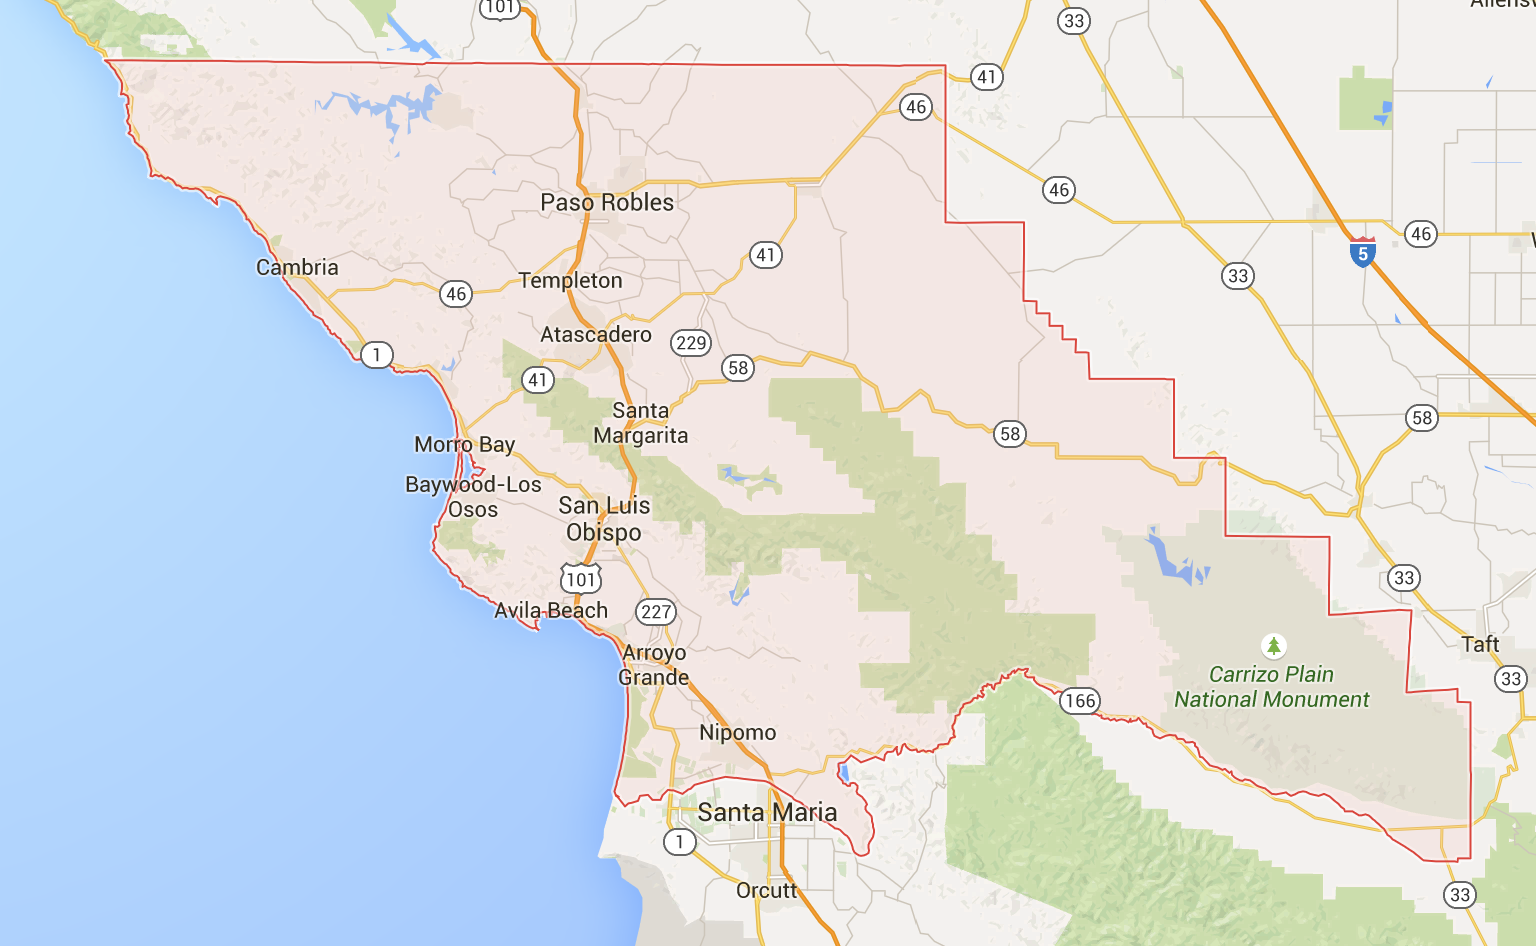
\includegraphics[width=0.84\textwidth]{figures/county.png}
    \caption{San Luis Obispo County lines. Note Paso Robles in the north. Pismo Beach (unlabeled) is between Avila Beach and Arroyo Grande}
    \label{fig:county}
\end{figure}

\begin{figure}
    \centering
    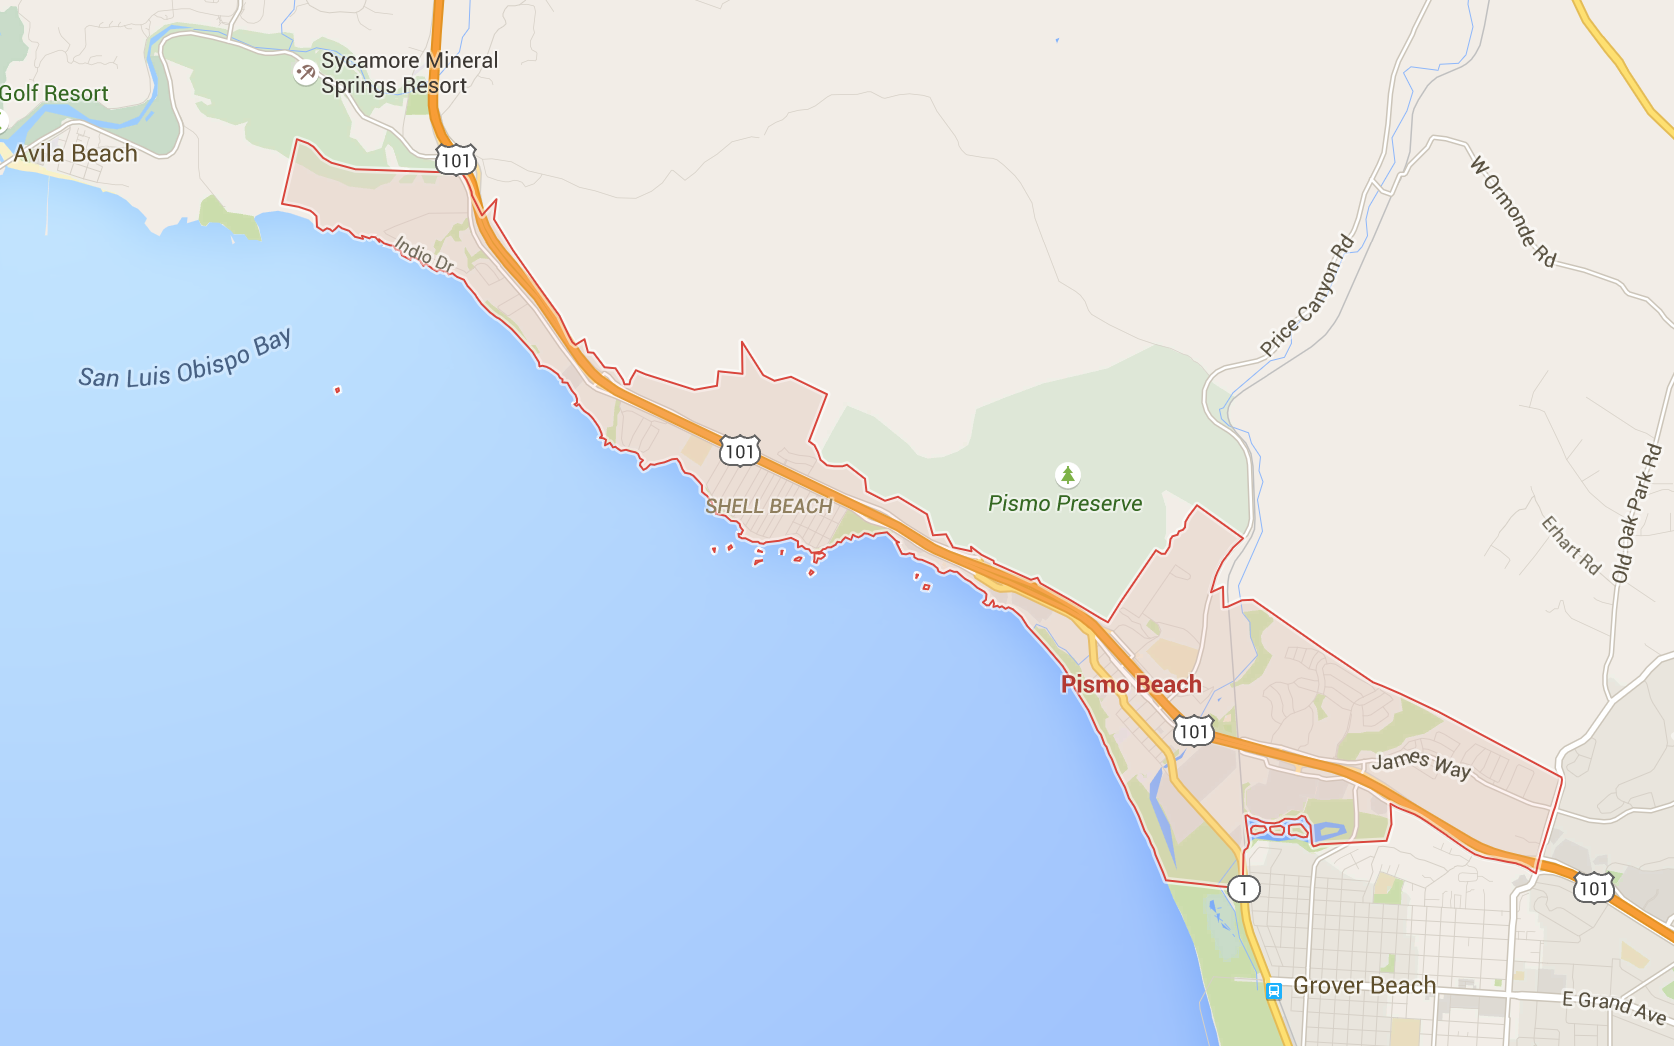
\includegraphics[width=0.87\textwidth]{figures/pismo.png}
    \caption{Pismo Beach city limits and pipeline region.}
    \label{fig:pismo}
\end{figure}

\begin{figure}
    \centering
    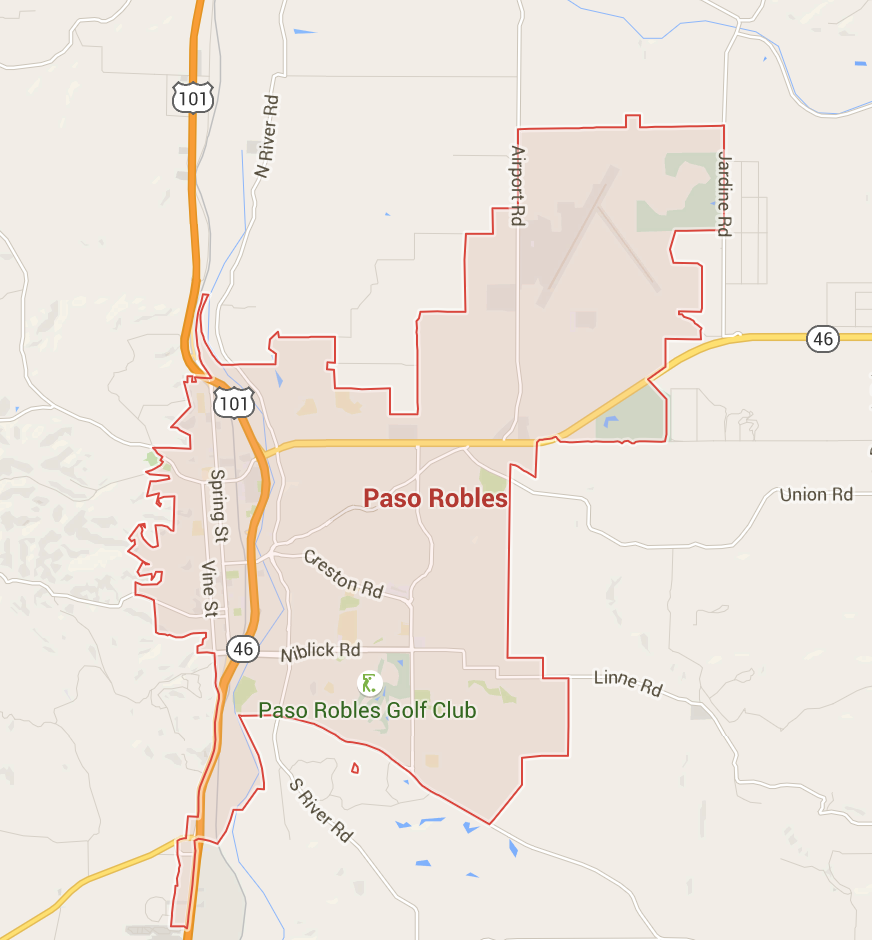
\includegraphics[width=0.55\textwidth]{figures/paso.png}
    \caption{Paso Robles city limits and pipeline region.}
    \label{fig:paso}
\end{figure}

The data from both organizations uses our permissioning system to allow shared, privileged access, as required by the business policies described below. Figure~\ref{fig:permissions} diagrams  
\begin{enumerate*}[label=\itshape\alph*\upshape)]
\item simple relationships between DataLayers and GeoViews and
\item the corresponding permissions setup for ABC Pipeline Co., XYZ Operations, and other RAPID users
\end{enumerate*}.

\begin{itemize}
\item As XYZ operates the Paso Robles pipeline on their own, they don't share the GeoView. The ground movement DataLayer is local and proprietary; they're sole Owner and Viewer. However, XYZ releases their rainfall DataLayer publicly, so that any RAPID user can view it.
\item Because ABC Pipeline Co. and XYZ Operations cooperate in the Pismo Beach pipeline region, ABC shares their relevant resources with XYZ: \begin{enumerate*}[label=\itshape\alph*\upshape)]
\item the county traffic DataLayer,
\item the Pismo Beach construction equipment DataLayer, and
\item the Pismo Beach GeoView
\end{enumerate*}.
\end{itemize}
 

\begin{figure}[h]
    \centering
    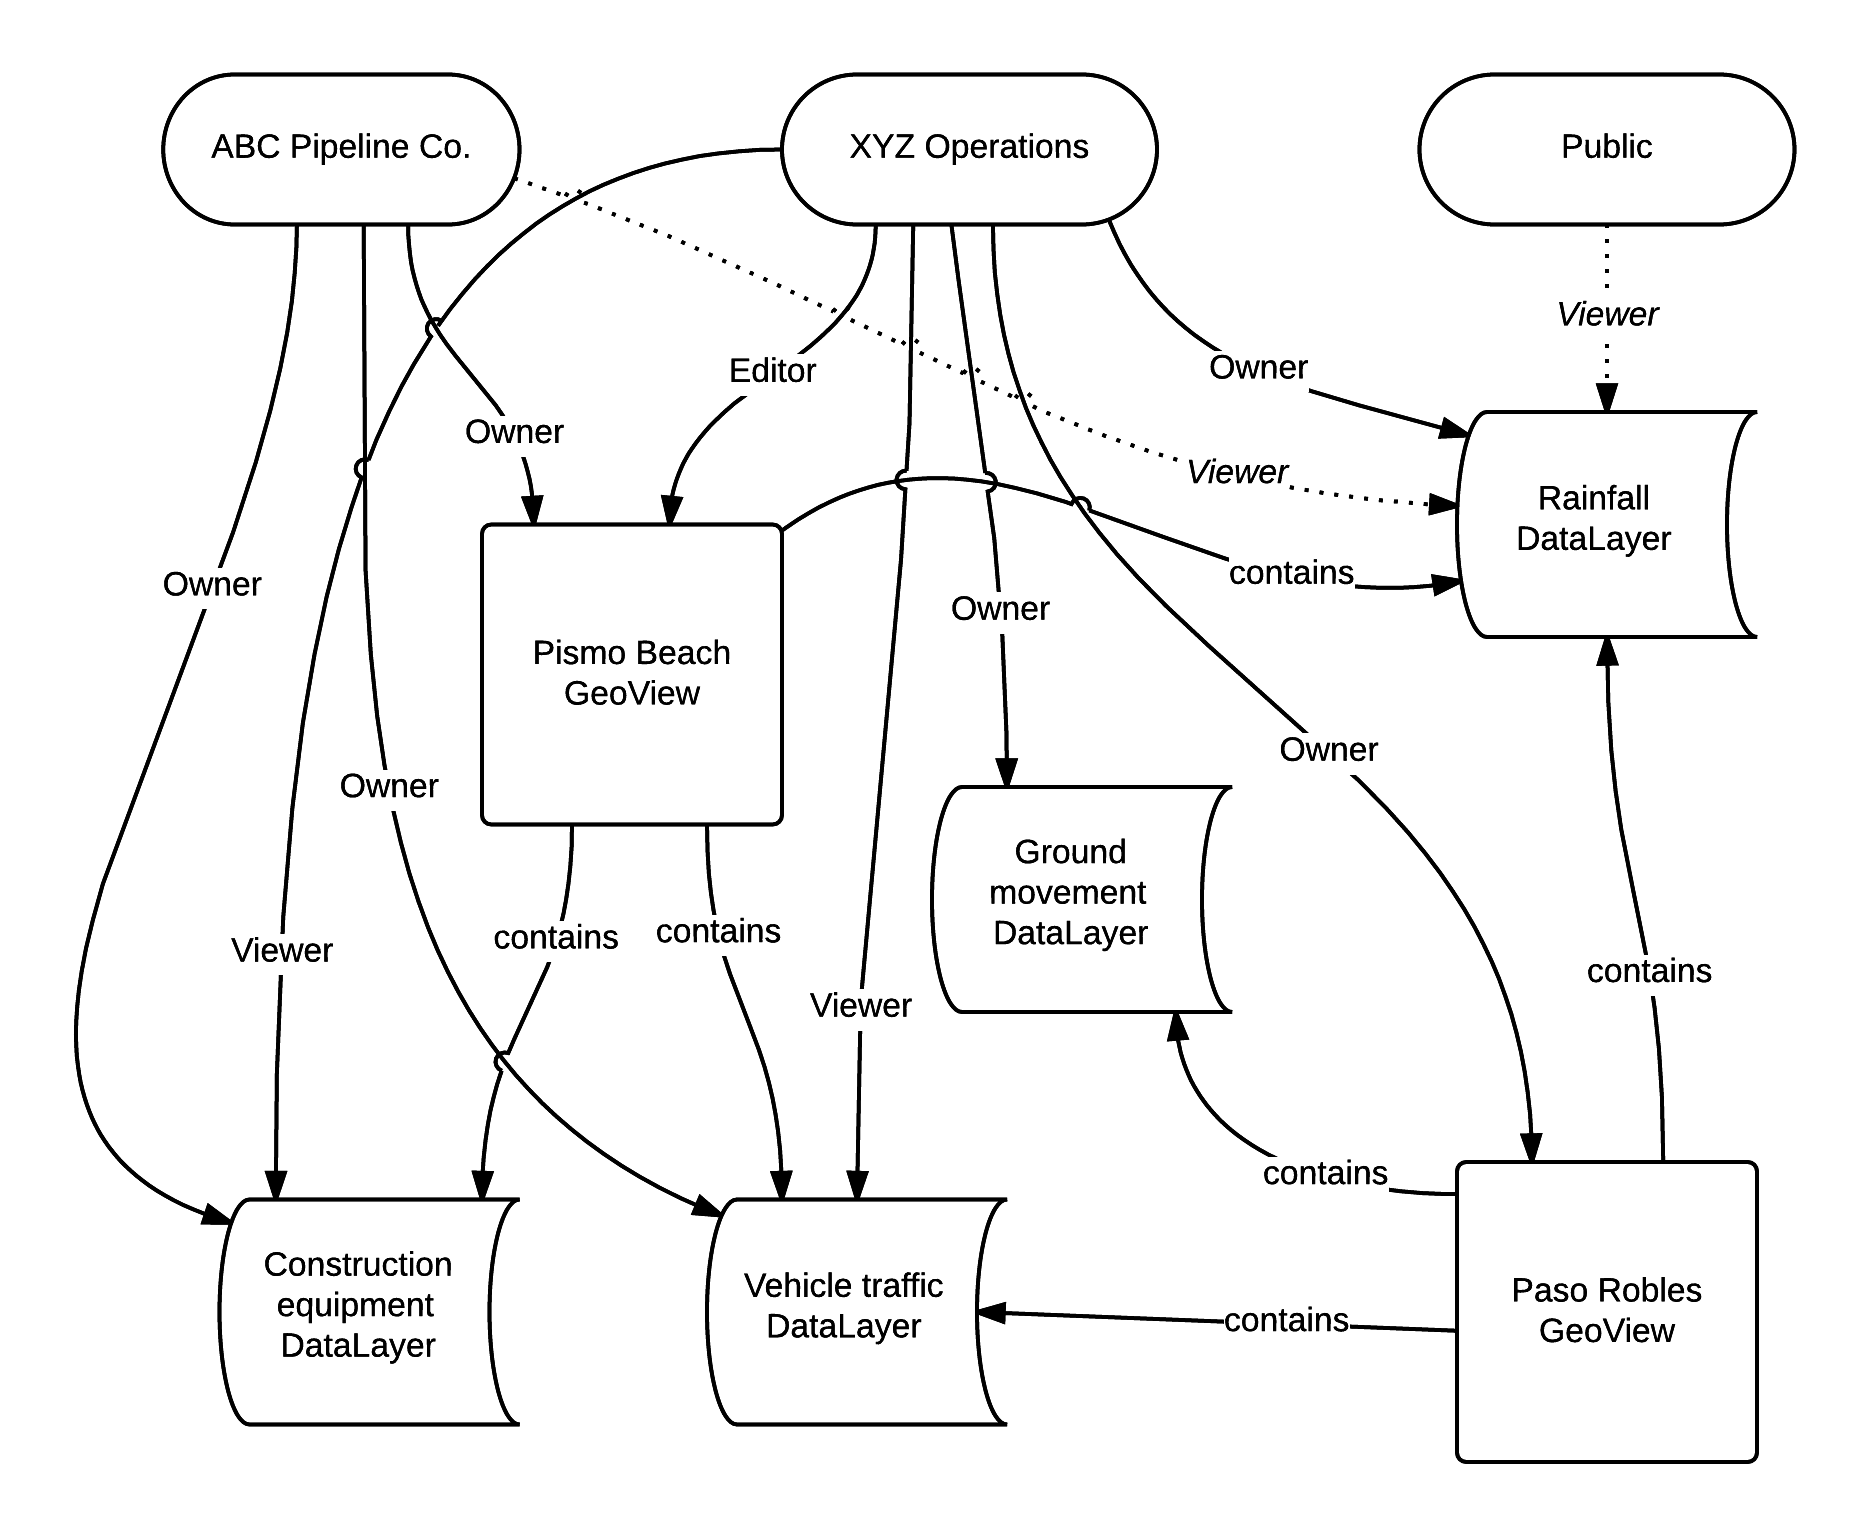
\includegraphics[width=0.99\textwidth]{figures/permissions.png}
    \caption{Example permissions setup between two organizations.}
    \label{fig:permissions}
\end{figure}

To slightly increase the complexity and realism of this example, we specify that the input formats begin as both GeoJSON and Shapefiles, and although ABC and XYZ review the same data for the same pipeline region, the groups use different DSS: ABC's only reads GeoJSON, and XYZ's only reads Shapefiles.

At a high level, with the above considerations, this scenario entails
\begin{enumerate*}[label=\itshape\alph*\upshape)]
\item setting up API tokens,
\item creating DataLayers,
\item importing GeoJSON and Shapefile features into DataLayers,
\item creating and querying GeoViews,
\item modifying permissions,
\item exporting data in GeoJSON and Shapefiles
\end{enumerate*}. Again note these are not always specific tasks for users---Francis describes those---but these end up being the most critical activities for our data model, described in the remainder of this chaper~\cite{Francis}. In other words, all of these can be accomplished by utilizing our models and writing queries with the techniques described in Section~\ref{sec:prog}, and following sections discuss specific class designs and source code that handle geospatial organization and querying. 

\begin{figure}[h]
    \caption{Entity-relationship diagram for RAPID's three primary geospatial classes.}
    \centering
    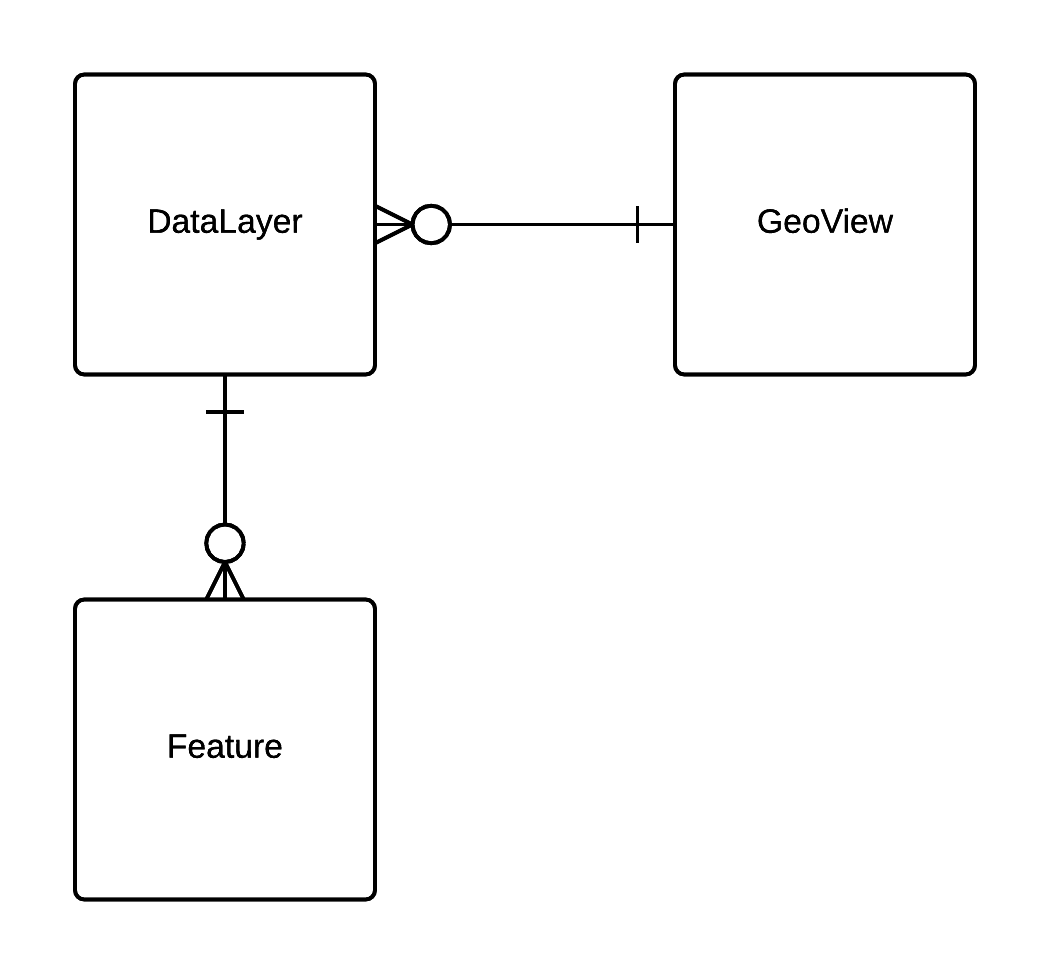
\includegraphics[width=0.5\textwidth]{figures/3er.png}
    \label{fig:3er}
\end{figure}

\section{Geospatial data modeling and organization}
Taken together, a small subset of RAPID classes enables structured data storage and retrieval for geographic features. In other words, these components could stand on their own, letting users browse and analyze geospatial objects (and groups of geospatial objects)---which fulfills our central database requirements. For the moment, we hold off discussing secondary functionality like permissioning, importing, and exporting data.

Figures~\ref{fig:feature},~\ref{fig:datalayer}, and~\ref{fig:geoview} show the relevant portions of our \texttt{models.py} file for the three models we've discussed throughout this paper. Figure~\ref{fig:3er}, shows a simple entity-relationship diagram to clarify the setup.

% archive = models.ForeignKey(Archive, null=True)

\begin{figure}
\caption{DataLayer class in models.py}
\begin{Verbatim}[samepage=true,baselinestretch=1,numbers=left,xleftmargin=12mm]
class DataLayer(models.Model):
    uid = models.TextField(unique=True, db_index=True)
    descriptor = models.TextField()
    properties = models.TextField(null=True)
    is_public = models.BooleanField(default=False)
\end{Verbatim}
\label{fig:datalayer}
\end{figure}

\begin{figure}
\caption{GeoView class in models.py}
\begin{Verbatim}[samepage=true,baselinestretch=1,numbers=left,xleftmargin=12mm]
class GeoView(models.Model):
    uid = models.TextField(unique=True, db_index=True)
    descriptor = models.TextField()
    geom = models.GeometryField(null=True)
    bbox = models.PolygonField(null=True)
    properties = models.TextField(null=True)
    layers = models.ManyToManyField('DataLayer', null=True)
\end{Verbatim}
\label{fig:geoview}
\end{figure}

\paragraph{Features}
We first describe the core makeup of \textit{features} in RAPID---that is, real geographic entities combined with other noteworthy indicators---and how they're presented to third parties. We saw in Chapter~\ref{background} that Geometry is the most generic and encompassing geospatial data type.\footnote{Remember that the Abstract Specification models these types hierarchically: a Polygon is a Polygon with holes, and a Polygon with holes is a Geometry, and so forth.} We also discussed that geospatial features correlate those mathematically-defined geometries with other descriptive attributes.

A RAPID Feature object is mostly a recreation of the geospatial features described in the Abstract Specification. There are some minor system-specific additions, but the purposes are similar enough that we borrow the terminology.

The Feature model comprises the following (with actual source code in Figure~\ref{fig:feature}):

\begin{description}
  \item[Geometry] \hfill \\
  A Geometry object represents the real-world footprint of the Feature (whether it's a Polygon, Line, Point, etc.). Functions from the OGC Standard can also be used to highlight various spatial characteristics like length, area, or circumference---calculations and descriptions people use everyday. Comparing two or more geometries (with the earlier-discussed relational operators) can reveal useful patterns, too.
   
   For simplicity, RAPID does not support elevations in a geometry. When importing Features, we only store the first two dimensions. This is usually fine for our pipeline operating partners: most relevant datasets are two-dimensional---the features are located on the Earth's surface (or at least within tens of feet).
   
   This missing third dimension is not related to the querying process (we never planned to allow Feature filtering based on height); it would only matter in data visualization or other analyses. In fact, three-dimensional geometry support is still rare in spatial DBMS (PostGIS is one of the only ones to actually support it). As an easy workaround on the user's end, the elevation could be ported rather easily to the Feature's properties, instead of residing in a Geometry.
  
  \item[Properties] \hfill \\
  Structured key-value stores are the norm for handling arbitrary GIS data, so an unlimited-length properties string bundles other relevant fields in a Feature. When shaping RAPID's usage style and conventions, we specifically wanted to support JSON as an intuitive data interchange format because our implementation leans on GeoJSON (and the REST API already parses JSON requests).
  
  The \texttt{properties} field introduces the ability to store and retrieve virtually any data for the Earth's surface (assuming it's serializable to JSON). Users that need extra functionality client-side can perform more advanced filtering and analysis with information besides just shape and location.
  
  \item[Unique identifier (UID)] \hfill \\
  We use a public, user-facing unique identifier (UID) for direct Feature lookups. While these could be any kind of unique value type, RAPID automatically generates textual UIDs upon Feature creation that are URL-safe and user-friendly (in that they're relatively short, using everyday numbers and letters).\footnote{We add UIDs to the three most prominent queryable models in RAPID---Feature, DataLayer, and GeoView---expecting that these are the objects under study and discussion. In that respect, the portability's very helpful.}\footnote{We coined this particular UID terminology for RAPID. An ``ID'' already gets used internally for back-end database work, and ``UUID'' (universally-unique identifier) is an existing standard for generating object identifiers~\cite{Leach}. Our UID makes use of the UUID standard behind the scenes, but they're not one and the same.} Because Features will often be retrieved using their UID, we add a database index for this field.
  
It's worth noting that our UIDs are generated randomly (with a secure random number generator) and end up being 22 bytes. An integer identifier would be reasonable too (especially with some slight indexing efficiencies over a longer string), but random strings won out:
  
  \begin{itemize}
  \item Features are the most numerous object type in RAPID. While we wouldn't expect to easily max out a 32- or 64-bit number, 22 bytes erases any worry of integer overflow when deployed over a wide area and many years.\footnote{The same argument could be made with fewer bytes: the library we're using happens to use 22.}
  \item We don't want identifiers to indicate ordering, magnitude, or chronology for Features: the UID should look more like a hash, as proximate integers could otherwise imply a relevant or analyzable relationship.
  \item Following that logic, a random string is helpful from a security standpoint. One organization could theoretically share UIDs for all their classified Features in the open, but no one else would be able determine how new, old, or similar they are through the UID. An incrementing counter could otherwise hint at those characteristics.
\end{itemize}
  
\item[Bounding box] \hfill \\
  It's somewhat common for GIS features to include a bounding box attribute---defining the minimally-bounding rectangle for the geometry. The small number of coordinates in a bounding box can estimate and rule out results in spatial functions more quickly than the ``true'' geometry.

  RAPID does not currently use bounding box checks (but they could be useful in the future, pending performance tests). However, bounding boxes are an important GIS topic in Simple Features Access, so we store them anyway~\cite{SFA}.
  
\item[Timestamp] \hfill \\
RAPID stores timestamps with Features---a filterable attribute when querying GeoViews---to indicate their relevance in time.

In a technical regard, \texttt{timestamp} is unremarkable, as it's simply another attribute to filter (as a range) when querying Features. However, as discussed in Chapter~\ref{background}, trend-watching is particularly useful and needed in GIS work. This timestamp lets pipeline operators and DSS find data that \begin{enumerate*}[label=\itshape\alph*\upshape)]
\item is most recent and applicable or
\item relevant for historical analyses
\end{enumerate*}.
  
\item[DataLayer foreign key] \hfill \\
A foreign key references the Feature's DataLayer---the DataLayers's \texttt{id}. Note that this is a many-to-one relationship (and the primary reason the relationship is directed from Feature to DataLayer). In other words, a Feature always has access to its DataLayer.

\textbf{Implementation note.} This one-way relationship, however, doesn't preclude us from traversing the relationship in the other direction---seeing all the Features for a DataLayer. That alternative action is common enough, and Django makes the querying easy: 

\begin{Verbatim}[samepage=true,baselinestretch=1,numbers=left,xleftmargin=12mm]
features = layer.feature_set
\end{Verbatim}

Even though a \texttt{feature\_set} isn't explicitly defined for a DataLayer, Django adds the property implicitly and handles the reverse lookup of the primary keys behind the scenes.

\end{description}

\paragraph{DataLayer}
DataLayers exist to usefully store multiple similarly-structured Features. Although there's a notion of layering in OGC standards, RAPID diverges from any of their detailed considerations and only keeps the spirit of categorization---hence the rename~\cite{AbstractSpecFaq,SFA,WFS}.

While RAPID doesn't enforce a consistent structure on properties, we'd expect them to be similar within a DataLayer so that they can be analyzed consistently. Although a misnomer, a DataLayer's Features might be imagined as \textit{instances} of the layer descriptor (see below), if they have similar schemas.

DataLayers start out with these fields:

\begin{description}

\item[UID] \hfill \\
DataLayers use the same UID construction as Features. While the larger string size isn't as necessary for the number of DataLayers as it is with Features---their count will never be the same order of magnitude---we keep the same setup for consistency. We could partially truncate the UID for DataLayers (and GeoViews) if we had to be extra concerned about it.

\item[Descriptor] \hfill \\
As a simple user-friendly and -facing title for DataLayers, we include a short Descriptor text field. The Descriptor labels the set of contained Features; ``Earthquake'' and ``Construction equipment'' are reasonable examples.

\item[Properties] \hfill \\
To mirror the properties capabilities in Features, we store JSON metadata in DataLayers (and leave it up to third parties to define the fields). Use of the metadata is optional, but it sometimes includes important documentation for Features' properties.

\item[Public flag] \hfill \\
When creating a DataLayer, we ask users to specify if it's a \textit{public} DataLayer, which anyone is allowed to view. For DataLayers that should be widely-accessible, this removes the inconvenience of adding a lot of Viewers manually. The original creator retains ownership and can continue to add other Owners and Editors as necessary (described later in this chapter).
  
\end{description}

 We haven't carried out performance testing to determine the tradeoffs, but we specifically chose \textit{not} to include bounding boxes on DataLayers, even though there \textit{could} be significant efficiency improvements to explore: one check with a DataLayer bounding box could avoid costly comparisons against thousands (or millions!) of Features. It'd be somewhat more complex, however, to keep the bounding dimensions up to date: as soon as Features change within a DataLayer, the bounding box must be recalculated.\footnote{The system design could have been set up to incorporate this, and there's an obvious place in the implementation to include the code, but it's outside our scope of work.}

\paragraph{GeoViews.}
It's possible (and reasonable) to retrieve all Features for a given DataLayer, but a more common and interesting use case lets users narrow the scope to a more precise and helpful dataset. This is shown explicitly with GeoViews---a way to retrieve data from combined DataLayers for a particular area. We, in fact, mostly expect applications to query GeoViews during daily operation---not DataLayers or Features---because they encompass a more complete study-able concept.

To elaborate, a GeoView includes 
\begin{enumerate*}[label=\itshape\alph*\upshape)]
\item one or more DataLayers and
\item a Geometry for a region of interest
\end{enumerate*}. RAPID saves which DataLayers are added to the view; when the GeoView is queried, Features from those DataLayers are returned to the requestor if they encroach on the chosen Geometry. GeoViews are rather analogous to ordinary SQL views (bringing about the name). They could even be implemented as them (aside from metadata), if so chosen.

To accommodate this functionality in the API, we define the GeoView model with these attributes:

\begin{description}

\item[DataLayer collection] \hfill \\
Each GeoView has a collection of the DataLayers to retrieve Features from. Users can add DataLayers to GeoViews (and remove them), so at run-time, their chosen DataLayers are searched.

\item[Geometry] \hfill \\
To indicate a specific physical location to query within or around, GeoViews include an assignable Geometry field. Early in requirements gathering, it was a forgone conclusion that GeoView Geometries narrow DataLayers to their specified region. That implied using the \texttt{Intersects} boolean relational operator so that all Features within or encroaching on a region are available. On the other hand, as RAPID's implementation progressed and API calls were tested, we noticed the value in supporting several of the Abstract Specification's spatial operators.

As such, \texttt{Intersects} is left as the default, but we also let callers to this interface choose \texttt{Contains} or \texttt{DWithin}. \texttt{Contains} produces of subset of the results of \texttt{Intersects}; the difference is that ``contained'' Features are \textit{fully} contained within the Geometry and cannot merely be overlapping the border. The \texttt{DWithin} operator produces a superset of Features from the \texttt{Intersects} results; the difference is Features within a certain distance of the Geometry are also selected. \texttt{DWithin} could highlight nearby Features that are still relevant (or that may be relevant in the future).

\item[Bounding box] \hfill \\
Again, pending performance tests, GeoView bounding boxes could prove to better our speeds, but they aren't currently set or used in our queries. We don't have the same concerns with bounding box consistency as we do with DataLayers, however, because there's only one geometry associated with the object.

\item[UID] \hfill \\
This identifier for GeoView rounds out our use of UIDs, included for the same reasons discussed in Features and DataLayers.

\item[Descriptor] \hfill \\
It makes sense for GeoView instances to have a user-friendly name to encompass their purpose---possibly shuffled among other GeoViews. An example we've seen would include ``Pismo Beach Pipeline.''

\item[Properties] \hfill \\
Included for the same reason in DataLayers, a properties field stores any desired metadata. In the case of GeoViews, users may want to provide detailed explanations on why the DataLayers are relevant or what different values indicate.

\end{description}

\textbf{Implementation note.} Django simply presents many-to-many relationships as collections in each model. Take the following example, where a DataLayer is added to a GeoView:

\begin{Verbatim}[samepage=true,baselinestretch=1,xleftmargin=12mm]
geoview.layers.add(layer)
\end{Verbatim}

Behind the scenes, Django creates and populates a junction table, mapping DataLayers to GeoViews (using their auto-generated primary keys).

\textbf{Example.} Instances of Features, GeoViews, and DataLayers.

\section{Importing and exporting data}
We can now describe how data is added to RAPID---how Features are ``imported'' from geospatial file formats---which might occur on-demand from API requests or at regular intervals automatically. We also take the opportunity to describe the export process.\footnote{Note that this only goes as far as to say how Features become and are converted from geospatial formats. The REST API itself includes other metadata and formatting in its requests and responses; the serialized geospatial file may be embedded in a larger JSON object~\cite{Francis}.} As we discussed in Chapter~\ref{design}, RAPID must read from and write to a variety of geospatial file formats (GeoJSON and Shapefiles at first). Here, we note how a user specifies a file and file type, and the generic process RAPID uses to parse and save Features. Although our requirements do specify GeoJSON and Shapefile support, we know other parsing capabilities may be required soon. As such, we've structured the objects and interfaces so that additional file formats will be easily importable at another time.\footnote{In general, we've looked to future-proof these high-level interfaces so that they're more dependent on the Abstract Specification than any one format or library.}

\subsection{Importing files}
The multiplicity of spatial and geographic file specifications is mirrored by the number of options in parsing, writing, validating, and transforming them. Some tools are easier to use than others; some support files that others don't. Some spatial DBMS will even handle encoding and decoding of popular formats natively. Therefore, we prioritize flexibility in the architecture for importing files and set up a pattern and process for consistent conversion.
 
In an \texttt{import.py} file, we add high-level file retrieval and parsing functionality, letting the API designate a file type and file location to import. As currently implemented, RAPID can parse GeoJSON and Shapefiles from a URL or on-disk file path. Once the file content is available, it's fed into a parser.\footnote{GeoJSON is an ordinary text-based file format, but as we discussed in Chapter~\ref{background}, Shapefiles are made of up multiple files, so they're transferred and stored as \texttt{.zip} files. Before parsing the extracted files, RAPID unzips this file.}

At a minimum, the parsing utilities and methods must extract geometries and key-value properties from the specified file content. With those available, they can be passed (along with the chosen DataLayer's UID) to our \texttt{create\_feature} function to handle final processing and . The property dictionary is converted to JSON; the geometry must end up in GeoJSON or WKT.\footnote{We don't dive into intricacies of file parsing and validation: official documentation and other tutorials provide the most accurate and proper guidelines. For example, we use GEOS for spatial data structures and operations, and python-geojson and PyShp for reading GeoJSON and Shapefiles~\cite{1,2,3}.}

Because multiple files can be added to one DataLayer, duplicate Features could be encountered; however, we need to eliminate redundancies so that these aren't interpreted as discrete entities. To address this, we add a hash value---a digest of the Feature---with the constraint that it is unique per DataLayer. In other words, any new features with precisely the same geometry and properties as an existing feature are disregarded.


\subsection{Exporting Features}
Exporting retrieved Features (maybe from queried GeoViews) works similarly to file importing (except in reverse), but it is primarily in the realm of Francis's API work~\cite{Francis}. To summarize, these are some of the critical steps and considerations:

\begin{itemize}
\item Blah 1
\item Blah 2
\end{itemize}

\section{Permission management}
Chapter~\ref{requirements} laid out permissioning capabilities for RAPID DataLayers and GeoViews. That functionality is enabled by adding several components. The entity-relationship diagram in Figure~\ref{fig:er} builds on the diagram in Figure~\ref{fig:3er}, showing the additional classes that make this an operational multi-tenant system.

\begin{figure}[ht]
    \centering
    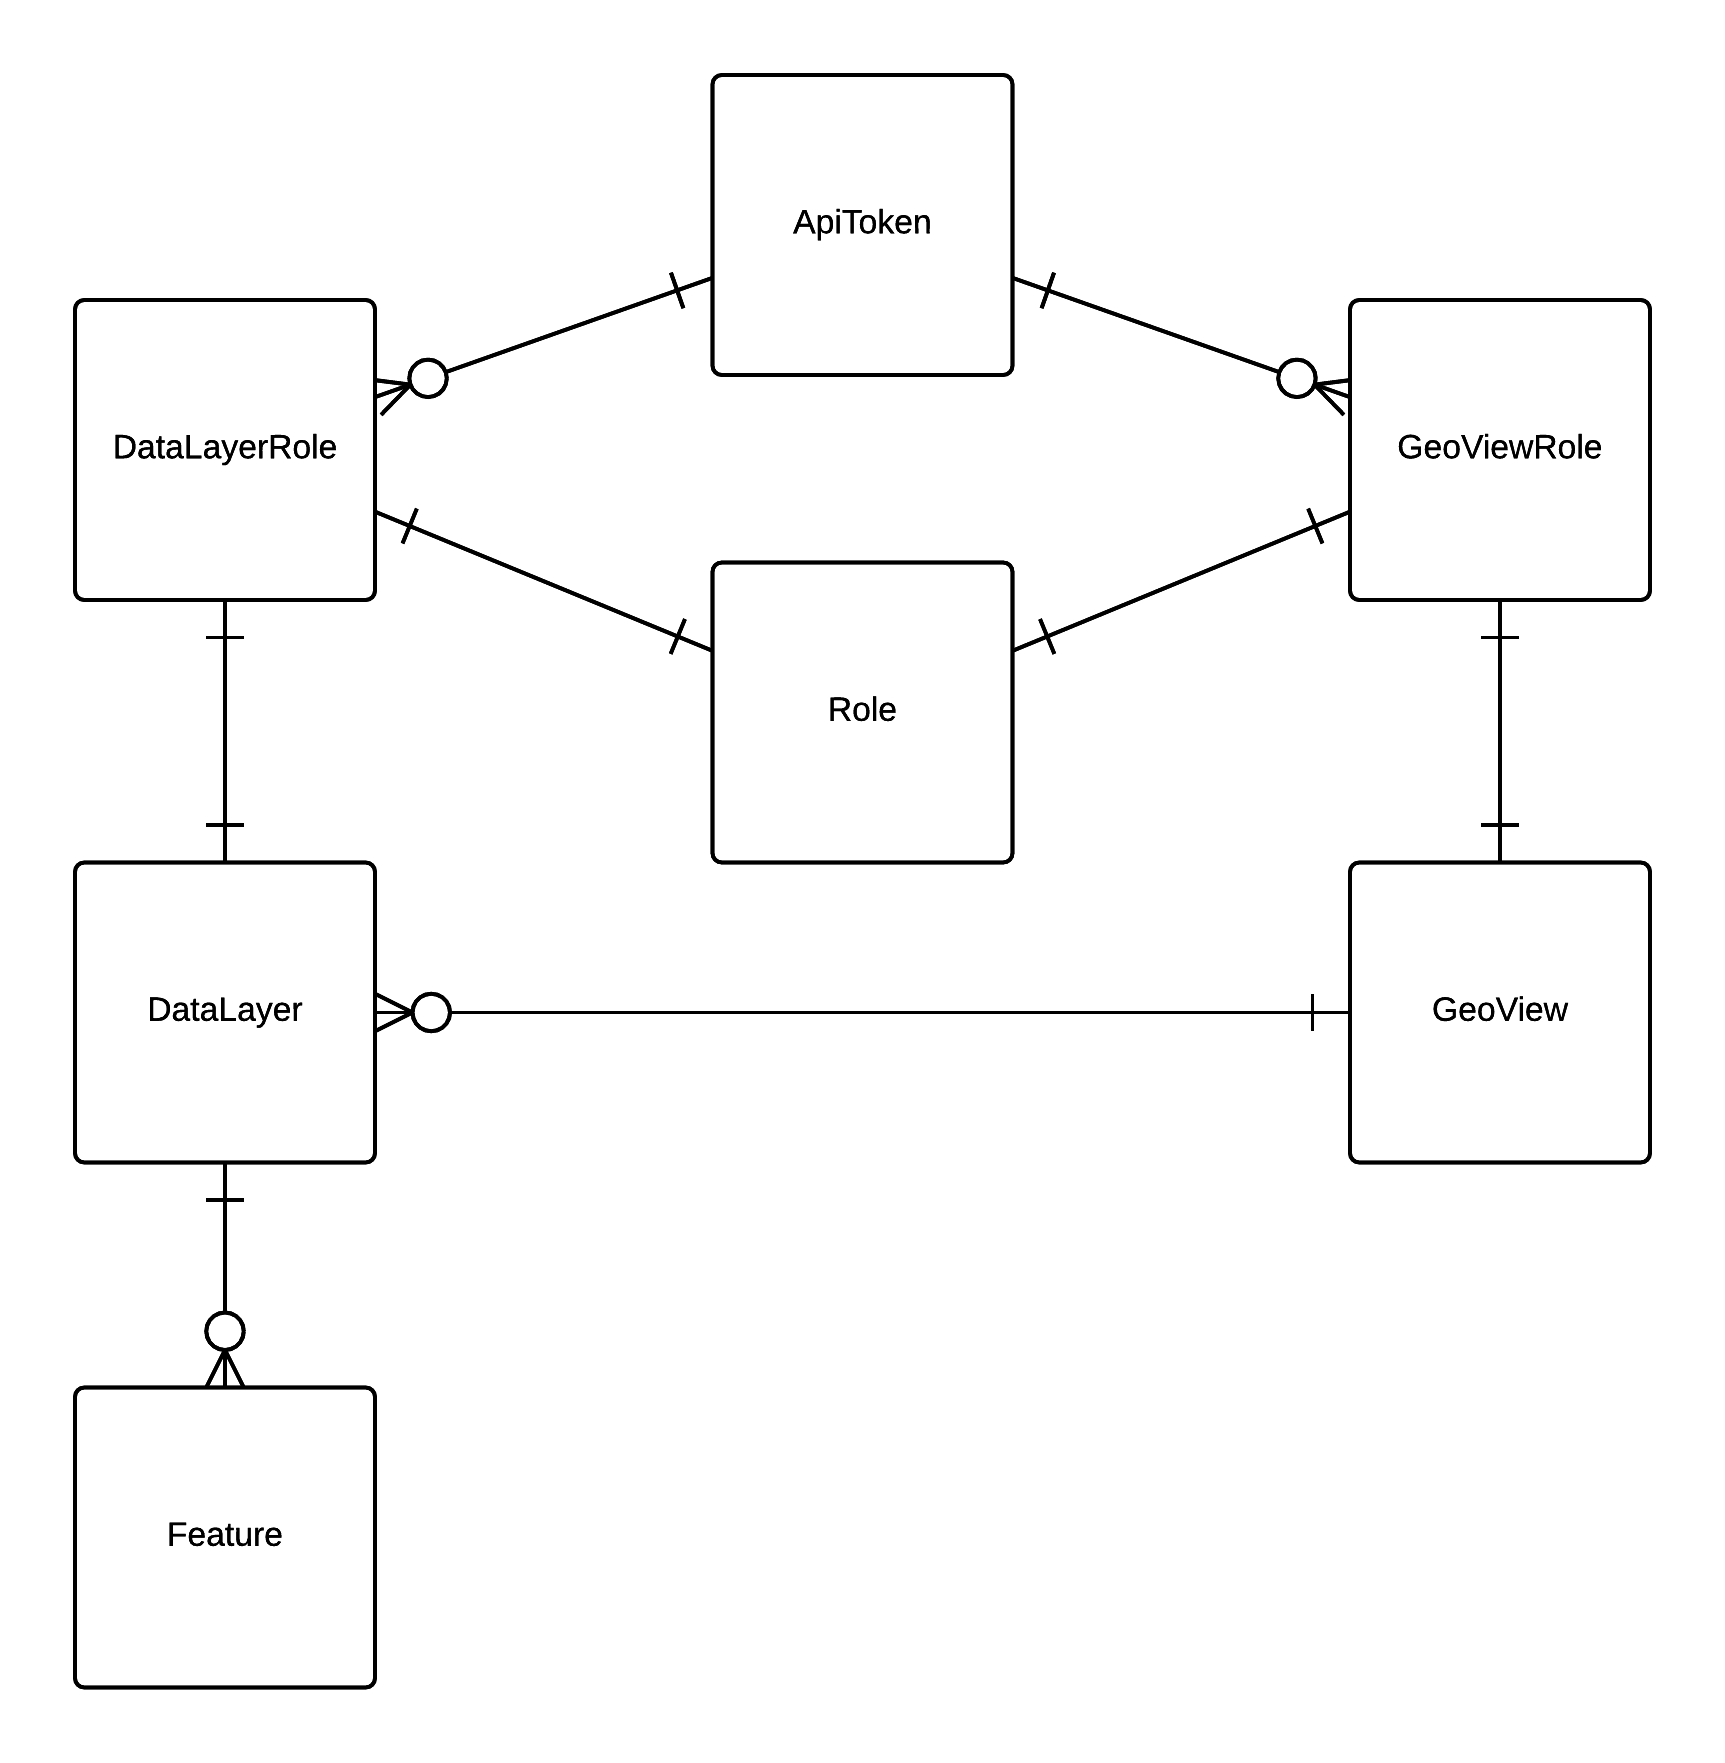
\includegraphics[width=0.99\textwidth]{figures/er.png}
    \caption{Entity-relationship diagram for RAPID's main conceptual data model, with permissioning capabilities.}
    \label{fig:er}
\end{figure}

\subsubsection{Role enum}
We add an enum, Role, to define the three available permission roles for RAPID data:
\begin{itemize}

  \item Owner
  \item Editor 
  \item Viewer
  \end{itemize}

Again recall that, on a daily basis, in-operation software is RAPID's end user: \textit{people} aren't necessarily Owners, Editors, or Viewers of data. We instead distribute API tokens that have assignable roles on each DataLayer and GeoView, and any system using that token has a uniform view of RAPID's resources.

\subsubsection{ApiToken}
The simple ApiToken model associates a friendly name (used as an identifier for administrative purposes) with a cryptographically-secure, randomly-generated key that grants resource access. When API requests come \textit{with} a token, RAPID knows who or what is requesting data and can return an appropriate set of results.


\begin{figure}
\begin{Verbatim}[samepage=true,baselinestretch=1,numbers=left,xleftmargin=12mm]
class ApiToken(models.Model):
    key = models.TextField(unique=True, db_index=True)
    descriptor = models.TextField(unique=True)
    issued = models.TimeField(null=True, auto_now_add=True)
\end{Verbatim}
\label{fig:apitoken}
\end{figure}

\begin{description}
\item[Name] \hfill \\
We require a friendly public name to identify this token. This can be used when choosing and assigning permissions for RAPID's other managed tokens.

\item[Key] \hfill \\
Upon creating an ApiToken and giving it a name, the system creates a long, random, URL-safe hash value to use as a password for sharing and accessing privileged data. When performing access-dependent API activities, the caller uses the (unguessable) token to show that they have the correct permissions, and RAPID checks the key against its internal records (the DataLayerRole and GeoViewRoles below).\footnote{While this setup is an accepted basis for web-based API security, RAPID should see an audit before storing truly classified data. For example, any other security measures are for naught if HTTPS is not enabled on the production server~\cite{Stormpath,Palmer}. }

\item[Timestamp] \hfill \\
Although our work is not focused on the security aspects of RAPID, we define and assign a creation timestamp for each token so that expiration or renewal policies can be implemented by future contributors.

\end{description}
To track newly-assigned permissions on DataLayers and GeoViews, we create DataLayerRole and GeoViewRole models, associating an ApiToken with a DataLayer or GeoView and specifying the particular role.


\begin{figure}
\begin{Verbatim}[samepage=true,baselinestretch=1,numbers=left,xleftmargin=12mm]
class GeoViewRole(models.Model):
    token = models.ForeignKey(ApiToken)
    role = enum.EnumField(Role)
    geo_view = models.ForeignKey(GeoView)
\end{Verbatim}
\label{fig:geoviewrole}
\end{figure}

\subsubsection{DataLayerRole and GeoViewRole}
\begin{description}
\item[ApiToken foreign key] \hfill \\
Specifies the ID of the ApiToken that has resource access.

\item[DataLayer or GeoView foreign key] \hfill \\
Specifies the ID of the DataLayer (if a DataLayerRole) or GeoView (if a GeoViewRole) to assign permissions to.

\item[Role enum] \hfill \\
The Role enum specifies the level of access this setup grants for the token on the chosen object.
\end{description}

% Could add user support to tokens down the road

\textit{[Integrate examples with ABC and XYZ's permissioning setup, showing specific roles and API tokens.]}


\label{design_srid}

\chapter{Implementation}
\label{implementation}

% We progress quickly through some sections of implementation: several modules are simply straightforward Python or SQL mappings from our data model and system design. 
\chapter{Validation}
\label{validation}
In this last chapter, we summarize our validation of RAPID, showing that the system meets Chapter~\ref{requirements}'s critical requirements, correctly uses the concepts and technologies outlined in our Background, and is efficient enough for real use in the future.

We made two primary contributions: 1) guidelines for API developers---at this point, Francis---and external partners to validate our data model and overall system design and 2) performance testing results for common operations.

\section{Functionality}
RAPID includes a geospatial data model as well as file parsing and querying capabilities. We must, therefore, verify that RAPID's design meets its specification and that our codebase parses, stores, queries, and outputs geospatial data correctly. These are particularly prudent, as RAPID's entire purpose is to enable portability and interchangeability for \textit{external} partners and \textit{future} developers.

Our example setup between ABC Pipeline Co. and XYZ Operations is a relatively complete case study, showing real class instances and relationships. By showing the models and implementation patterns in Chapter~\ref{design} that support that needed functionality, it should be apparent that RAPID completely and successfully meets our system requirements in Chapter~\ref{requirements}.

Even though our model is, hopefully, convincing on its own, we worked with another student developer, Kishan Patel, to integrate a web application with RAPID for further validation. We call this software \textit{RAPID UI}, which visualizes spatial entities and our organization of data (Features in DataLayers, DataLayers grouped into GeoViews).

Our peer developer, Patel, had to become acquainted with basic geospatial concepts and client-side libraries, but our contributions to RAPID were significant and successful enough that he was able to create a sensible UI using our most important API calls. Second, being able to visualize our data---both geographic geometries and accompanying properties---we can literally see that data makes it through RAPID, from beginning to end, as expected. As an additional nicety, we share and visualize several datasets with RAPID UI that were recently recommended by pipeline operating partners.

Francis describes our work with Patel in-depth---she also worked with him to design and fully test REST calls---but please see the following, where we outline our expectations and findings for RAPID UI, focusing on the data model's relevance.

\begin{itemize}
\item A primary goal in researching GIS standards and technologies was to ensure RAPID operates as expected when handling (rather finicky) geospatial data. Therefore, we set up several sample DataLayers for RAPID UI

So, of important note, Patel uses

\item Helo
\end{itemize}

\section{Performance}
The previous section shows that, given our data model and business logic, RAPID operates properly; we now use this section to highlight our core data model's performance, showing that it's an efficient base for future additions. We point out specific interface actions from earlier that typify DSS work and compare their runtimes.

\subsection{Setup and results}
\textit{[Finish this section.]}
% db_index on off.

small, medium, large
points, polygons
Specific features
DataLayer lookup
GeoView lookup


\subsection{Unit testing discussion}
% All of these components could be validated with a thorough unit test suite, using these recommendations. On the back end, RAPID uses the Django web framework, which utilizes Python's standard library testing module, \texttt{unittest}~\cite{DjangoTesting}. Once each necessary data field is accounted for in each possible input and output format, exhaustive unit tests can ensure that each field in one format can be converted to the corresponding field in every other format.

% \begin{itemize}
% \item Writable and parseable digital format like GeoJSON or Shapefile.
% \item In-memory objects.
% \item WKT or GeoJSON---abstract text formats for geospatial features.
% \item Abstract data added to and retrieved from PostGIS.
% \end{itemize}

% Data can move linearly up and down that list; each of those steps and transitions can also be viewed as a data integrity checkpoint that deserves a unit test. For instance, a Polygon made up of bordering points (0, 0), (0, 10), and (10, 0) still needs to have the same meaning---a triangle with those three points---no matter where its format or location. GeoJSON files and Shapefiles, Python objects, WKT or GeoJSON notation, and PostGIS data structures can all be inspected to ensure that the same data is contained in each. If it isn't, the data was misshaped somewhere along the line that can be traced.

\clearpage
\begin{flushleft}
% \nocite{*}
\bibliography{bibliography}
\bibliographystyle{plain}
\end{flushleft}

\begin{appendices}
\input{appendix-outline}
\end{appendices}

\end{document}